% !TeX spellcheck = en_GB

\documentclass[proc]{edpsmath}
\usepackage[utf8]{inputenc}
\usepackage[T1]{fontenc}
%\usepackage{microtype}

\usepackage{amsmath,amssymb,amsthm}
%\usepackage{graphicx}
%\usepackage{bbold}
%\usepackage{enumerate}
\usepackage{hyperref}
\usepackage{physics}
%\usepackage{float} 
%\usepackage{mathtools}
%\mathtoolsset{showonlyrefs=true}
%\usepackage{tikz}

\newcommand{\bR}{\mathbb{R}}
\newcommand{\bb}{\mathbf{b}}
\newcommand{\bA}{\mathbf{A}}
\newcommand{\vp}{v_\parallel}
\newcommand{\bx}{\mathbf{x}}
\newcommand{\bv}{\mathbf{v}}
\newcommand{\bu}{\mathbf{u}}
\newcommand{\bB}{\mathbf{B}}
\newcommand{\Dt}{\Delta t \;}

\newcommand{\dbx}{\dot{\mathbf{x}}}
\newcommand{\diff}[2]{\frac{\text{d} #1}{\text{d} #2}}
\newcommand{\pa}[2]{\frac{\partial #1}{\partial #2}}
\newcommand{\ap}{a_\parallel}
\newcommand{\mean}[1]{\langle #1 \rangle}
\newcommand{\Bap}{B_\parallel^\ast}
\newcommand{\bracket}[2]{\left\{ #1, #2 \right\}}
\newcommand{\gcbracket}[2]{\left\{ #1, #2 \right\}_{\text{g.c.}}}
\newcommand{\dt}{\frac{\text{d}}{\text{d} t}}

\renewcommand{\d}{\;\text{d}}


\begin{document}

\title{SILAS - Semi-Lagrangian scheme with Arakawa splitting}
\thanks{CEMRACS}\thanks{Max-Planck}% At most 5 thanks
%
\author{Dominik Bell}\address{Max-Planck-Institut für Plasmaphysik, Garching, Germany; \email{dominik.bell@ipp.mpg.de\ \&\ frederik.schnack@ipp.mpg.de\ \&\ martin.campos-pinto@ipp.mpg.de\ \&\ sonnen@ipp.mpg.de}}\secondaddress{Technische Universität München, Zentrum Mathematik, Garching, Germany}
\author{Martin Campos Pinto}\sameaddress{1}
\author{Vador Mukozec}\address{Faculty of Sciences, University of Novi Sad, Serbia; \email{davor.kumozec@dmi.uns.ac.rs}}
\author{Frederik Schnack}\sameaddress{1}
\author{Eric Sonnendrücker}\sameaddress{1,2}

\begin{abstract}
In practice, there are various ways to solve gyro-kinetic equations. Here we will combine the Semi-Lagrangian (SL) and Arakawa scheme. Both schemes are successfully implemented in practice when applied individually, but our goal is to decompose the problem into fast (parallel) dynamic and slow (perpendicular) dynamic and to combine these two schemes. SL scheme will be used to solve fast subsystem and Arakawa scheme for slow. In \cite{pygyro_code}, what is our reference code, the entire model is solved using SL, and we will replace the part related to the slow subsystem with an Arakawa scheme. The main reason for combining these two schemes is to get a solution that preserves some of the basic measures in the system we have. In Section II we will describe properties of both schemes and splitting between advection equations. In Part III numerical experiments will be presented, first for Arakawa scheme as verification of theoretical properties and after that for PyGyro model.
\end{abstract}
%
\begin{resume}
En pratique, il existe différentes manières de résoudre les équations gyro-cinétiques. Ici, nous allons combiner le schéma Semi-Lagrangien (SL) et Arakawa. Les deux schémas sont mis en œuvre avec succès dans la pratique lorsqu'ils sont appliqués individuellement, mais notre objectif est de décomposer le problème en dynamique rapide (parallèle) et dynamique lente (perpendiculaire) et de combiner ces deux schémas. Le schéma SL sera utilisé pour résoudre le sous-système rapide et le schéma Arakawa pour le lent. Dans \cite{pygyro_code}, quel est notre code de référence, tout le modèle est résolu à l'aide de SL, et nous remplacerons la partie liée au sous-système lent par un schéma d'Arakawa. La principale raison de combiner ces deux schémas est d'obtenir une solution qui préserve certaines des mesures de base du système que nous avons. Dans la section II, nous décrirons les propriétés des deux schémas et la séparation entre les équations d'advection. Dans la partie III, des expériences numériques seront présentées, d'abord pour le schéma d'Arakawa comme vérification des propriétés théoriques et ensuite pour le modèle PyGyro.
\end{resume}


\maketitle

\tableofcontents %TODO: can also be removed later


\section{Introduction}

\textbf{Strang splitting} is a numerical tool which can be used in numerical computation of PDEs, coupled together with the \textbf{Lie splitting} gives us the resulting equations which are much simpler for solving with reasonable error (for more details see [emily thesis]). In our equation 
\begin{equation}
 \partial_t f + \{\phi, f \} + v_\parallel \nabla_\parallel f - \nabla_\parallel \phi\,\, \partial_{v_\parallel} f = 0
\end{equation}
for distribution function $f$ we can split numerical computations into three advection equations:
\begin{equation}
 \partial_t f + v_\parallel \nabla_\parallel f = 0 \qquad \text{Advection on flux surface}
\end{equation}
\begin{equation}
 \partial_t f + \nabla_\parallel \phi\,\, \partial_{v_{\parallel}} f = 0 \qquad \text{V-parallel advection}
 \end{equation}
\begin{equation}
 \partial_t f + \{\phi, f\} = 0 \qquad \text{Advection on poloidal plane}
\end{equation}
where $\{\phi,f\}$ is a Poisson bracket, defined as follows:
\begin{equation}
 \{\phi,f\}=-\frac{\partial_\theta\phi}{rB_0}\partial_r f + \frac{\partial_r\phi}{rB_0}\partial_\theta f.
\end{equation}
In our work, we will use two different approaches to solving these three equations. For the first two we will use the semi-Lagranzian scheme and for the third Arakawa scheme.

\subsection{Semi-Lagrangian scheme for fast time subsystem}
The fast time subsystem will be solved using semi-Lagrangian scheme. As reference we will use \cite{campospinto} and [emily thesis]. The code for this part can be found at \cite{pygyro_code}. To begin with, we will use general notations and then we will move on to the problem we have in our model. This scheme is frequently used in solving advection problems of the form:

\begin{equation}
    \partial_t f(t,\mathbf{x})+v(t,\mathbf{x})\cdot \nabla f(t,\mathbf{x})=0, \qquad t\in[0,T], \quad \mathbf{x}\in\mathbb{R}^d
\end{equation}
where $v$ is a velocity field $\mathbb{R}^d\longrightarrow\mathbb{R}^d$, $T$ is a final time and initial conditions is given by $f_0(\mathbf{x})=f(0,\mathbf{x})$. For the simplicity, we will assume that $v$ is given and smooth enough so we can use method of characteristics. Let say that under the smooth assumptions we have trajectories $X(t)=X(t;s,x)$ which are obtained as a solution to ODE
\begin{equation}
    X'(t)=v(t,X(t)), \qquad X(s)=x, \qquad t\in[0,T].
\end{equation}
It can be shown that the flow $F_{s,t}:x\longrightarrow X(t)$ is invertible and satisfies $(F_{s,t})^{-1}=F_{t,s}$. We know that analytical solution to our equation is given by
\begin{equation}
    f(t,\mathbb{x})=f_0((F_{0,t})^{-1}(x)),\qquad \text{for } t\in[0,T], \quad \mathbf{x}\in\mathbb{R}^d.
\end{equation}
Now we are using backward tracking of the characteristic
\begin{equation}
    B^{n,n+1}=(F_{t_n,t_{n+1}})^{-1}
\end{equation}
between two time steps $t_n=n\Delta t$ and $t_{n+1}$. For the last step we have to approximate function $f$ at grid points $f^n=f(t_n)$. For this purpose, we will use splines.\\
The flux surface advection operator defined by equation
\begin{equation}
 \partial_t f + v_\parallel \nabla_\parallel f = 0
\end{equation}
is a two-dimensional semi-Lagrangian operator. Here we can determine the exact trajectory because the velocity in the equation is constant and is not related to the surface of the flux.\\
In order to determine the value of the distribution function in the discretization grid for characteristics that go outside our domain, we use a combination of a one-dimensional cubic spline and a Lagrangian interpolation polynomial of the fifth order in the $\theta$ and $z$ directions, respectively. In this way, we get an approximation of the value of the function in the final position.\\
The v$_\parallel$ surface advection operator defined by equation
\begin{equation}
    \partial_t f + \nabla_\parallel \phi\,\, \partial_{v_{\parallel}} f = 0
\end{equation}
is a one-dimensional semi-Lagrangian operator and here we use a cubic spline to determine the value of the particle distribution function for characteristics that go outside the domain. The parallel gradient $\phi$ depends only on the spatial coordinates and is therefore constant along the surface v$_\parallel$. As a result, the trajectory used by the semi-Lagrangian method can be accurately defined. The parallel gradient $\phi$ is computed using 6th-order finite differences (field-aligned) in the $z$ direction. This was calculated as described by Latu et al. \cite{Latu_2017}.

\subsection{Arakawa scheme for slow time subsystem}

For the Arakawa scheme, we mainly reference the article \cite{Arakawa_1966}. Here we are interested in solving the advection on poloidal plane:
\begin{equation}
 \partial_t f + \{\phi, f\} = 0
\end{equation}
where $\{\phi,f\}$ is a Poisson bracket, defined as follows:
\begin{equation}
 \{\phi,f\}=-\frac{\partial_\theta\phi}{rB_0}\partial_r f + \frac{\partial_r\phi}{rB_0}\partial_\theta f.
\end{equation}
The Arakawa scheme provably preserves the following quantities:
	\begin{align*}
		\text{mass} : && \dt \int f(t) \d x \text{d} y & = 0 & \Leftrightarrow && \int\bracket{\phi}{f} \d x \text{d} y & = 0 \\
		L^2\text{-norm :} && \dt \int f^2(t) \d x \text{d} y & = 0 & \Leftrightarrow && \int f \, \bracket{\phi}{f} \d x \text{d} y & = 0 \\
		\text{total energy :} && \dt \int \phi \, f(t) \d x \text{d} y & = 0 & \Leftrightarrow && \int \phi \bracket{\phi}{f} \d x \text{d} y & = 0
	\end{align*}
First we will focus on discretization of Poisson bracket in Cartesian coordinates. The scheme in polar coordinates is analogous.\\

\textbf{The main idea of Arakawa scheme - construction of the 4th order bracket approximation:}\\
The first step in constructing the 4th order Arakawa scheme is to explain second order discretization using nine point stencil. We have approximation of $J(f,g)$ at $(i,j)$ of the following form
\begin{equation}
J(f,g)=\frac{1}{3}(J^{++}+J^{+\times}+J^{\times+})+\mathcal{O}(d^2)
\end{equation}
where
\begin{equation}
    J^{++}_{ij}=\frac{1}{4d^2}[(f_{i+1,j}-f_{i-1,j})(g_{i,j+1}-g_{i,j-1})-(f_{i,j+1}-f_{i,j-1})(g_{i+1,j}-g_{i-1,j})],
\end{equation}
\begin{equation}
    J^{+\times}_{ij}=\frac{1}{4d^2}[f_{i+1,j}(g_{i+1,j+1}-g_{i+1,j-1})-f_{i-1,j}(g_{i-1,j+1}-g_{i-1,j-1})-f_{i,j+1}(g_{i+1,j+1}-g_{i-1,j+1})+f_{i,j-1}(g_{i+1,j-1}-g_{i-1,j-1})]
\end{equation}
and
\begin{equation}
    J^{\times+}_{ij}=\frac{1}{4d^2}[f_{i+1,j+1}(g_{i,j+1}-g_{i+1,j})-f_{i-1,j-1}(g_{i-1,j}-g_{i,j-1})-f_{i-1,j+1}(g_{i,j+1}-g_{i-1,j})+f_{i+1,j-1}(g_{i+1,j}-g_{i,j-1})]
\end{equation}
We denote the linear combination $J_1=\frac{1}{3}(J^{++}+J^{+\times}+J^{\times+})$, which is a second order approximation conserving the square of vorticity and the energy.\\
In order to extend discretization to 4th order we introduce $J_2=\frac{1}{3}(J^{\times \times}+J^{\times+}+J^{+\times})$ where we use the same nine point stencil with the additional
four points $(i+2,j)$, $(i-2,j)$, $(i,j+2)$  and $(i,j-2)$ for $J_2$, where
\begin{equation}
    J^{\times\times}_{ij}=\frac{1}{8d^2}[(f_{i+1,j+1}-f_{i-1,j-1})(g_{i-1,j+1}-g_{i+1,j-1})-(f_{i-1,j+1}-f_{i+1,j-1})(g_{i+1,j+1}-g_{i-1,j-1})]
\end{equation}
\begin{equation}
    J^{\times+}_{ij}=\frac{1}{8d^2}[f_{i+1,j+1}(g_{i,j+2}-g_{i+2,j})-f_{i-1,j-1}(g_{i-2,j}-g_{i,j-2})-f_{i-1,j+1}(g_{i,j+2}-g_{i-2,j})+f_{i+1,j-1}(g_{i+2,j}-g_{i,j-2})],
\end{equation}
and
\begin{equation}
    J^{+\times}_{ij}=\frac{1}{8d^2}[f_{i+2,j}(g_{i+1,j+1}-g_{i+1,j-1})-f_{i-2,j}(g_{i-1,j+1}-g_{i-1,j-1})-f_{i,j+2}(g_{i+1,j+1}-g_{i-1,j+1})+f_{i,j-2}(g_{i+1,j-1}-g_{i-1,j-1})].
\end{equation}
By Taylor extension, we can see that $2J_1-J_2$ is a fourth order approximation of the Jacobian $J$; that is,
$2J_1-J_2=J+O(d^4)$.
Now we have the second-order nine-point
scheme and the fourth-order thirteen-point scheme. For the proof of the stencil order, we refer to appendix \ref{sec:ara_order}.\\

\noindent
\textbf{Boundary Conditions}\\
Let show first what is happening if $g$ is constant at boundary. By
\begin{equation}
    J_{ij}(f,g)=\sum^*_{i',j'}[a_{i,j;i+i',j+j'}(f_{i+i',j+j'}+f_{i,j})-a_{i-i',j-j';i,j}(f_{i,j}+f_{i-i',j-j'})].
\end{equation}
and assume g is constant at the boundary j = 0 (and outside of domain), the discrete Jacobi is treated as
\begin{equation}
\begin{aligned}
\frac{1}{2}J_{i0} (f,g) &= a_{i,0;i+1,0}(f_{i+1,0}+f_{i,0})-a_{i-1,0;i,0}(f_{i-1,0}+f_{i-1,0})\\
&-\frac{1}{12d^2}[(g_{i+1,0}+g_{i+1,1}-g_{i-1,0}-g_{i-1,1})(f_{i,0}+f_{i,1})\\
&+(g_{i+1,0}-g_{i,1})(f_{i,0}+f_{i+1,1})\\
&+(g_{i,1}-g_{i-1,0})(f_{i-1,1}+f_{i,0})].
\end{aligned}
\end{equation}
We need to keep f constant case (stationary state), so it holds that $$\sum_{i',j'} a_{i,j;i+i',j+j'}=0.$$ 
Then 
$$a_{i,0;i+1,0}-a_{i-1,0;i,0}-\frac{1}{12d^2}(2g_{i+1,0}-2g_{i-1,0}+g_{i+1,1}-g_{i-1,1})=0.$$
Rewrite it as 
$$a_{i,0;i+1,0}-\frac{1}{12d^2}(g_{i,1}+g_{i+1,1}-g_{i,0}-g_{i+1,0})=a_{i-1,0;i,0}-\frac{1}{12d^2}(g_{i-1,1}+g_{i,1}-g_{i-1,0}-g_{i,0}).$$
Right hand side has the same formula with left hand side by replacing i by i-1. Each term is not depend on i, so it is constant. Because this term $a_{i,0;i+1,0}(f_{i+1,0}+f_{i,0})-a_{i-1,0;i,0}(f_{i-1,0}+f_{i-1,0})$ is a approximation of $-\partial_y g \partial_x f$ on the boundary, so the constant is 0.
At last, we have $$a_{i,0;i+1,0}=\frac{1}{12d^2}(g_{i,1}+g_{i+1,1}-g_{i,0}-g_{i+1,0})$$ and $$a_{i-1,0;i,0}=\frac{1}{12d^2}(g_{i-1,1}+g_{i,1}-g_{i-1,0}-g_{i,0}).$$ 
That is,
\begin{equation}
\begin{aligned}
\frac{1}{2}J_{i0} (f,g) &=-\frac{1}{12d^2}[(-g_{i,1}-g_{i+1,1}+g_{i,0}+g_{i+1,0})(f_{i+1,0}+f_{i,0})\\
&-(-g_{i-1,1}-g_{i,1}+g_{i-1,0}+g_{i,0})(f_{i-1,0}+f_{i,0})\\
&+(g_{i+1,0}+g_{i+1,1}-g_{i-1,0}-g_{i-1,1})(f_{i,0}+f_{i,1})\\
&+(g_{i+1,0}-g_{i,1})(f_{i,0}+f_{i+1,1})\\
&+(g_{i,1}-g_{i-1,0})(f_{i-1,1}+f_{i,0})].
\end{aligned}
\end{equation}
Similarly, we obtain the scheme for boundary $j=J$:
\begin{equation}
\begin{aligned}
\frac{1}{2}J_{iJ} (f,g) &=-\frac{1}{12d^2}[(g_{i,J-1}+g_{i+1,J-1}-g_{i,J}-g_{i+1,J})(f_{i+1,J}+f_{i,J})\\
&-(g_{i-1,J-1}+g_{i,J-1}-g_{i-1,J}-g_{i,J})(f_{i-1,J}+f_{i,J})\\
&-(g_{i+1,J}+g_{i+1,J-1}-g_{i-1,J}-g_{i-1,J-1})(f_{i,J}+f_{i,J-1})\\
&-(g_{i+1,J}-g_{i,J-1})(f_{i,J}+f_{i+1,J-1})\\
&-(g_{i,J-1}-g_{i-1,J})(f_{i-1,J-1}+f_{i,J})].
\end{aligned}
\end{equation}
The discrete integral constraint $gf$ is $$\sum_{i}[ \frac{1}{2}g_{i,0}J_{i0}+\sum_{j=1}^{J-1} g_{i,j}J_{ij}+\frac{1}{2}g_{i,J}J_{iJ}].$$

\begin{remark}
For second order Arakawa scheme with g Dirichlet boundary condition, we can take $g_{i,0}=g_{i,-1}$ as a constant. However we can't directly modify fourth order scheme in this way by taking $g_{i,0}=g_{i,-1}=g_{i,-2}$ since the coefficients  $a_{i,0;i,-1}=\frac{1}{8d^2}(g_{i-1,1}-g_{i+1,0})$ and $a_{i,0;i+1,-1}=\frac{-1}{8d^2}(g_{i+1,1}-g_{i-1,0})$ (from $J^{\times \times}$) are not 0, so that we can't use half stencil. If we use half stencil, the coefficients can not be balanced, so we can't keep the conservation. 
\end{remark}

\noindent
If function $f$ is constant at boundary: By $J_{ij}=-J_{ji}$, exchanging the position of f and g, we can get the scheme for the boundary f constant case:

for $j=0$:

\begin{equation}
\begin{aligned}
\frac{1}{2}J_{i0} (f,g) &=\frac{1}{12d^2}[(-f_{i,1}-f_{i+1,1}+f_{i,0}+f_{i+1,0})(g_{i+1,0}+g_{i,0})\\
&-(-f_{i-1,1}-f_{i,1}+f_{i-1,0}+f_{i,0})(g_{i-1,0}+g_{i,0})\\
&+(f_{i+1,0}+f_{i+1,1}-f_{i-1,0}-f_{i-1,1})(g_{i,0}+g_{i,1})\\
&+(f_{i+1,0}-f_{i,1})(g_{i,0}+g_{i+1,1})\\
&+(f_{i,1}-f_{i-1,0})(g_{i-1,1}+g_{i,0})].
\end{aligned}
\end{equation}

for $j=J$:

\begin{equation}
\begin{aligned}
\frac{1}{2}J_{iJ} (f,g) &=\frac{1}{12d^2}[(f_{i,J-1}+f_{i+1,J-1}-f_{i,J}-f_{i+1,J})(g_{i+1,J}+g_{i,J})\\
&-(f_{i-1,J-1}+f_{i,J-1}-f_{i-1,J}-f_{i,J})(g_{i-1,J}+g_{i,J})\\
&-(f_{i+1,J}+f_{i+1,J-1}-f_{i-1,J}-f_{i-1,J-1})(g_{i,J}+g_{i,J-1})\\
&-(f_{i+1,J}-f_{i,J-1})(g_{i,J}+g_{i+1,J-1})\\
&-(f_{i,J-1}-f_{i-1,J})(g_{i-1,J-1}+g_{i,J})].
\end{aligned}
\end{equation}

\textbf{Extrapolation at boundary for the 4th order Arakawa}\\
It is easy to get 4th order convergence, but how about conservation properties?

\textbf{Arakawa with homogeneous dirichlet boundary}\\
In \cite{crouseilles2018exponential}, they show that the mass of Arakawa scheme for dirichlet boundary is not conserved up to machine precision, even for homogeneous Dirichlet boundary conditions. By their numerical experiments, the Arakawa scheme works better for homogeneous boundary condition. In their test, they assume that $f(r_{min}, \theta,z,v)=f_{eq}(r_{min},v)$ and $f(r_{max}, \theta,z,v)=f_{eq}(r_{max},v)$ but not homogeneous Dirichlet boundary. In addition to the direct formulation, we can also introduce a so-called perturbation formulation by dividing f into $f=f_{eq}+\delta f(t,r,\theta,v)$. With this formulation, our model problem can be written as 
\begin{equation}
 \partial_t \delta f + \{\phi, \delta f \} + v_\parallel \nabla_\parallel \delta f - \nabla_\parallel \phi\,\, \partial_{v_\parallel} \delta f + \{\phi, \delta f_{eq} \}= 0,
\end{equation} 
which is similar as our model problem. The Arakawa scheme that is used to discretize $\{\phi, \delta f \}$ now employs homogeneous Drichlet boundary conditions for $\delta f$ in r-direction.

% !TeX spellcheck = en_GB


\section{Numerical Experiments}



\subsection{Pure Advection}








\subsection{PyGyro}

Our main point of comparing the Arakawa method to the Semi-Lagrangian scheme are the conserved quantities: the mass
\begin{equation}
	\int f(r, \theta, z, v_\parallel) \d r \d \theta \d z \d v_\parallel
\end{equation}
and $l^2$-norm
\begin{equation}
	\left[\int f^2(r, \theta, z, v_\parallel) \d r \d \theta \d z \d v_\parallel\right]^\frac{1}{2}
\end{equation}
of the distribution function, and the potential energy
\begin{equation}
	\int \left(f(r, \theta, z, v_\parallel) - f_\text{eq}(r, v_\parallel)\right) \Phi(r, \theta, z) \d r \d \theta \d z \d v_\parallel
\end{equation}
, as well as the not necessarily conserved kinetic energy
\begin{equation}
	\int \left(f(r, \theta, z, v_\parallel) - f_\text{eq}(r, v_\parallel)\right) v^2_\parallel \d r \d \theta \d z \d v_\parallel
\end{equation}

From a simulation with grid size $[r:128, \theta:256, z:128, v_\parallel :72]$ and time step-size $\Delta t = 1$ we plot for the above mentioned 4 quantities the absolute error (figure \ref{fig:abserr}), the relative error (figure \ref{fig:relerr}), and the relative error on a logarithmic scale (\ref{fig:relerrlog}) before and after the poloidal advection step.

We can clearly see that the Arakawa scheme preserves the conserved quantities much better than semi-Lagrangian scheme. In the linear phase, the error is of order of machine precision. Only very late in the non-linear phase becomes the relative error bigger, but is still one or two orders of magnitude smaller than in the semi-Lagrangian scheme.

The kinetic energy is also much better preserved.

The same study with time-step size $\Delta t = 2$ was done (figures \ref{fig:abserr_dt2}, \ref{fig:relerr_dt2}, \ref{fig:relerrlog_dt2}) and yields the same results. It is therefore interesting to compare the results of the poloidal advection step for the Arakawa method for the two time step-sizes; these results are shown in figures \ref{fig:abserr_akw}, \ref{fig:relerr_akw}, \ref{fig:relerrlog_akw}. We see that the doubling of the time step-size results in double the absolute error for the conserved quantities, and about a factor of 5 for the kinetic energy.

\begin{figure}
	\centering
	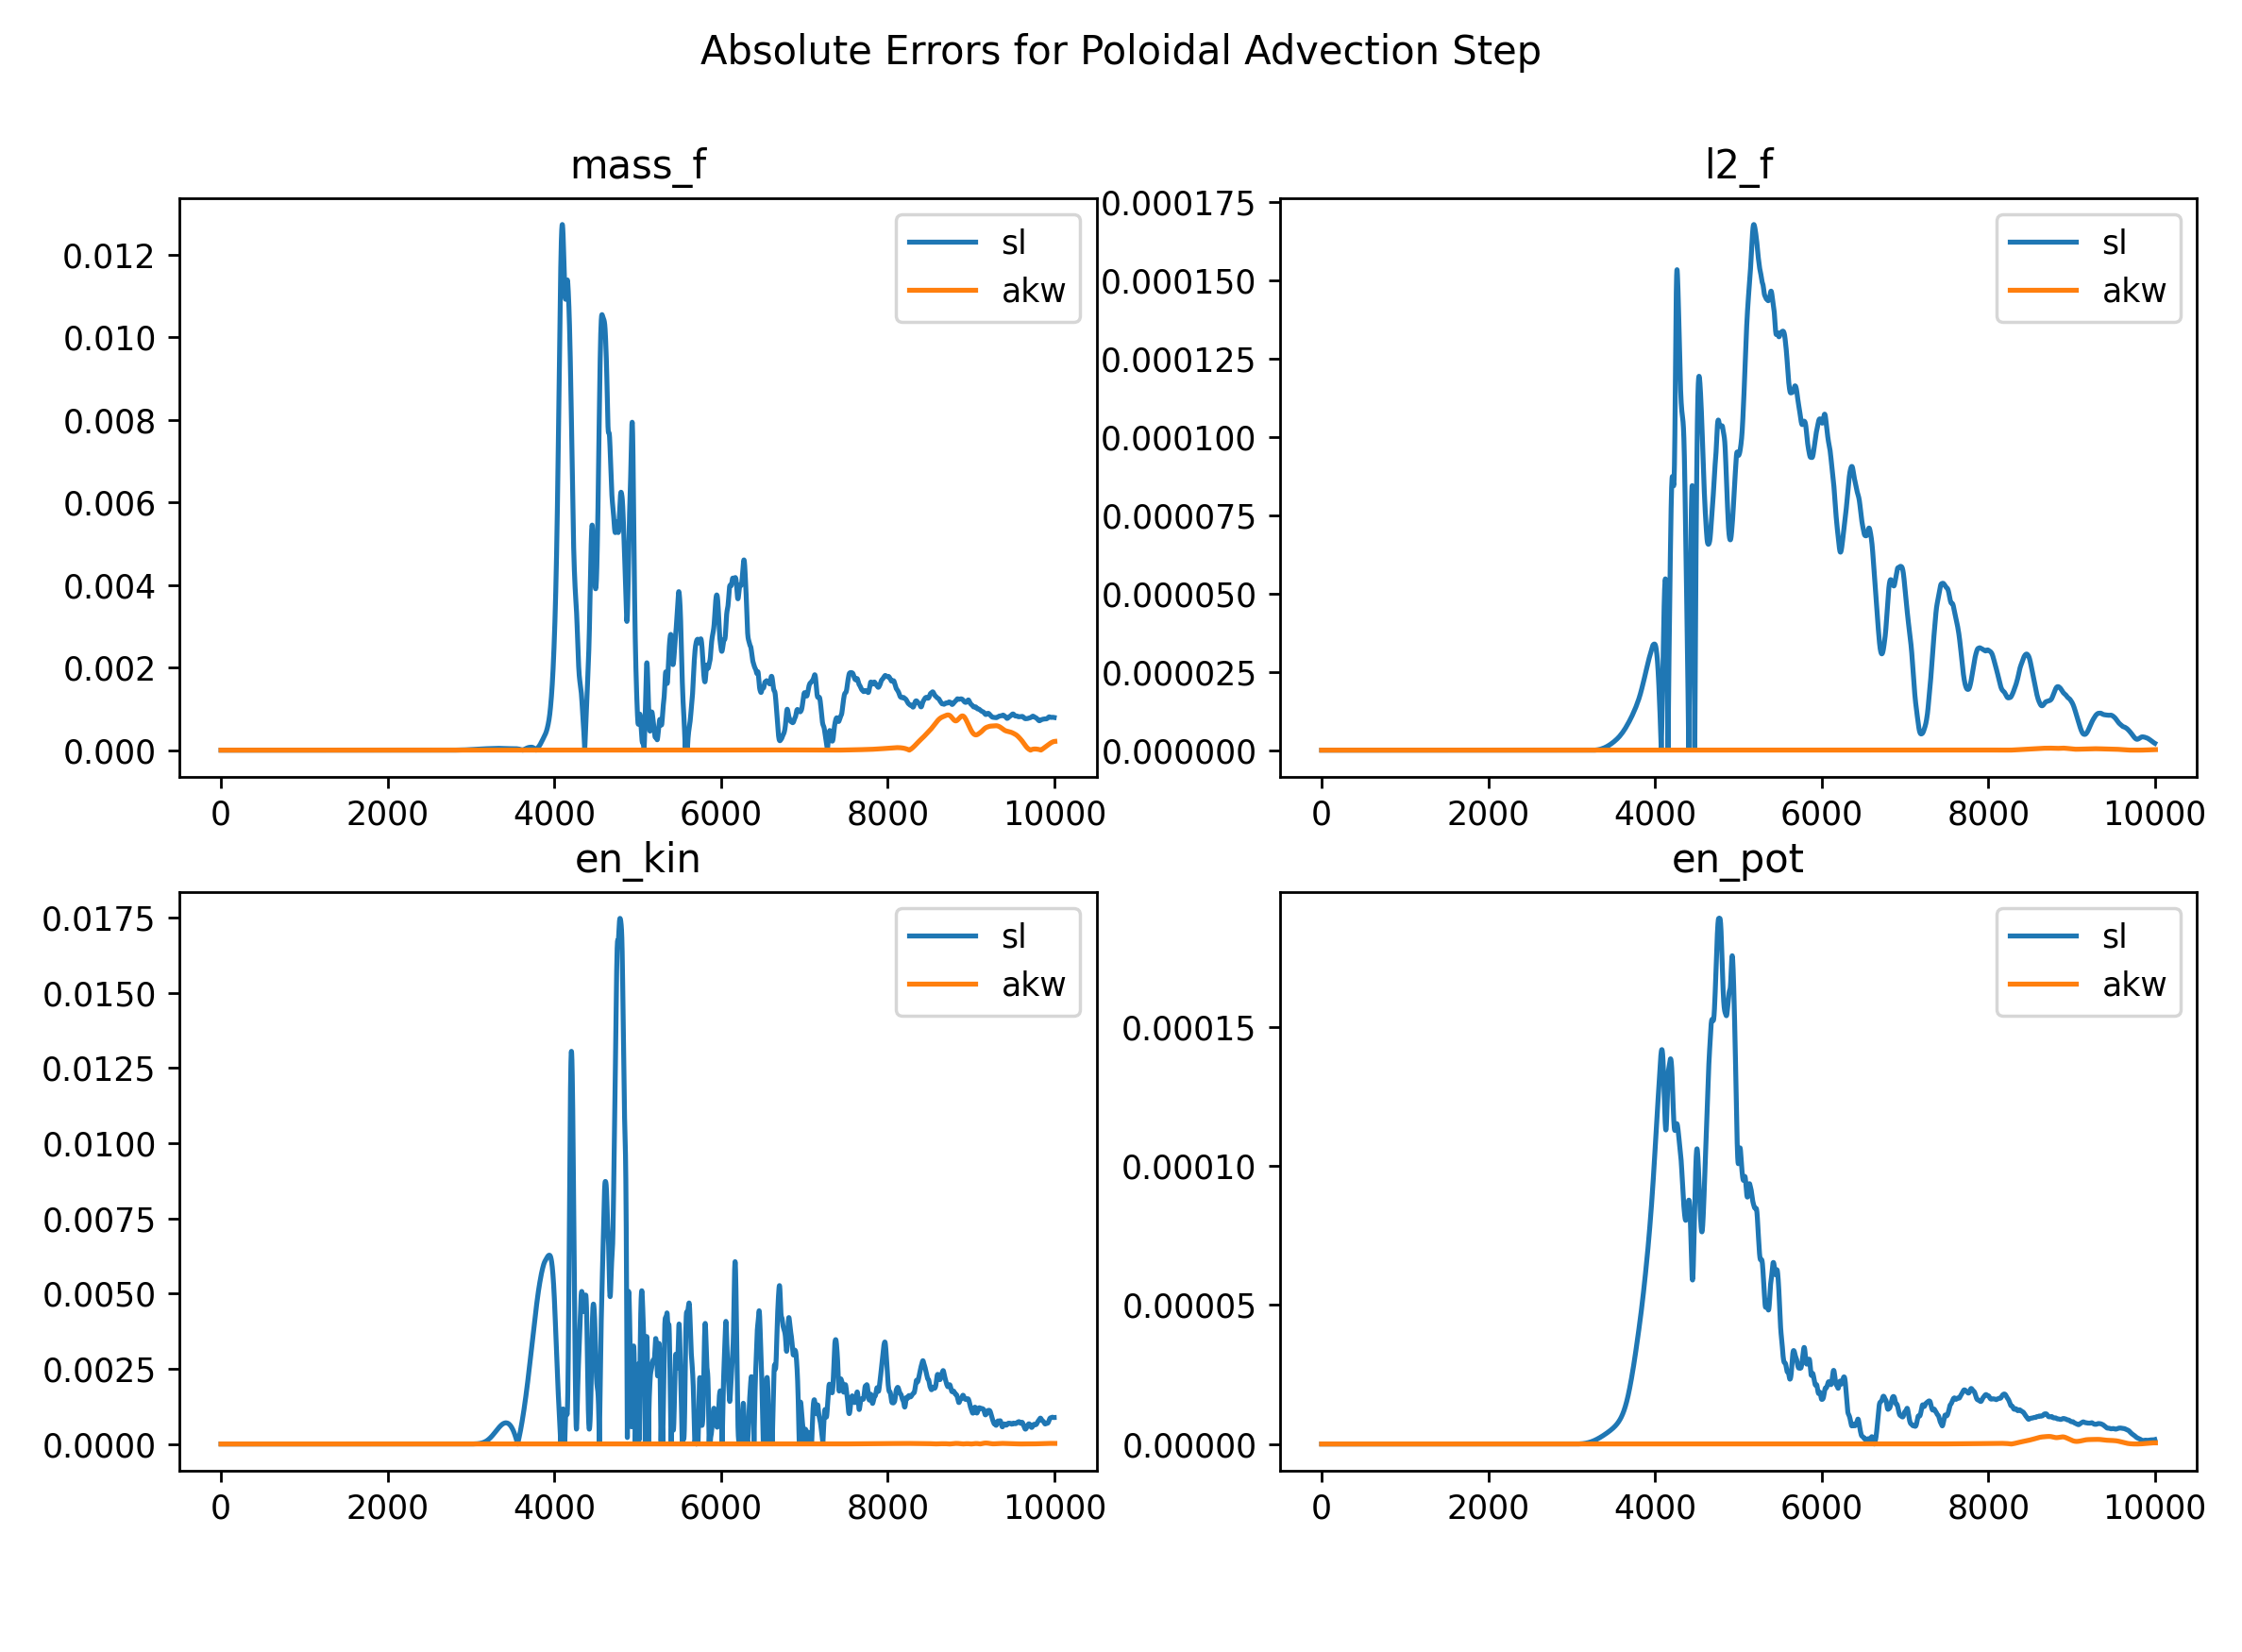
\includegraphics[width=0.9\linewidth]{plots/abs_err}
	\caption{The absolute error for different quantities before and after the poloidal advection step.}
	\label{fig:abserr}
\end{figure}


\begin{figure}
	\centering
	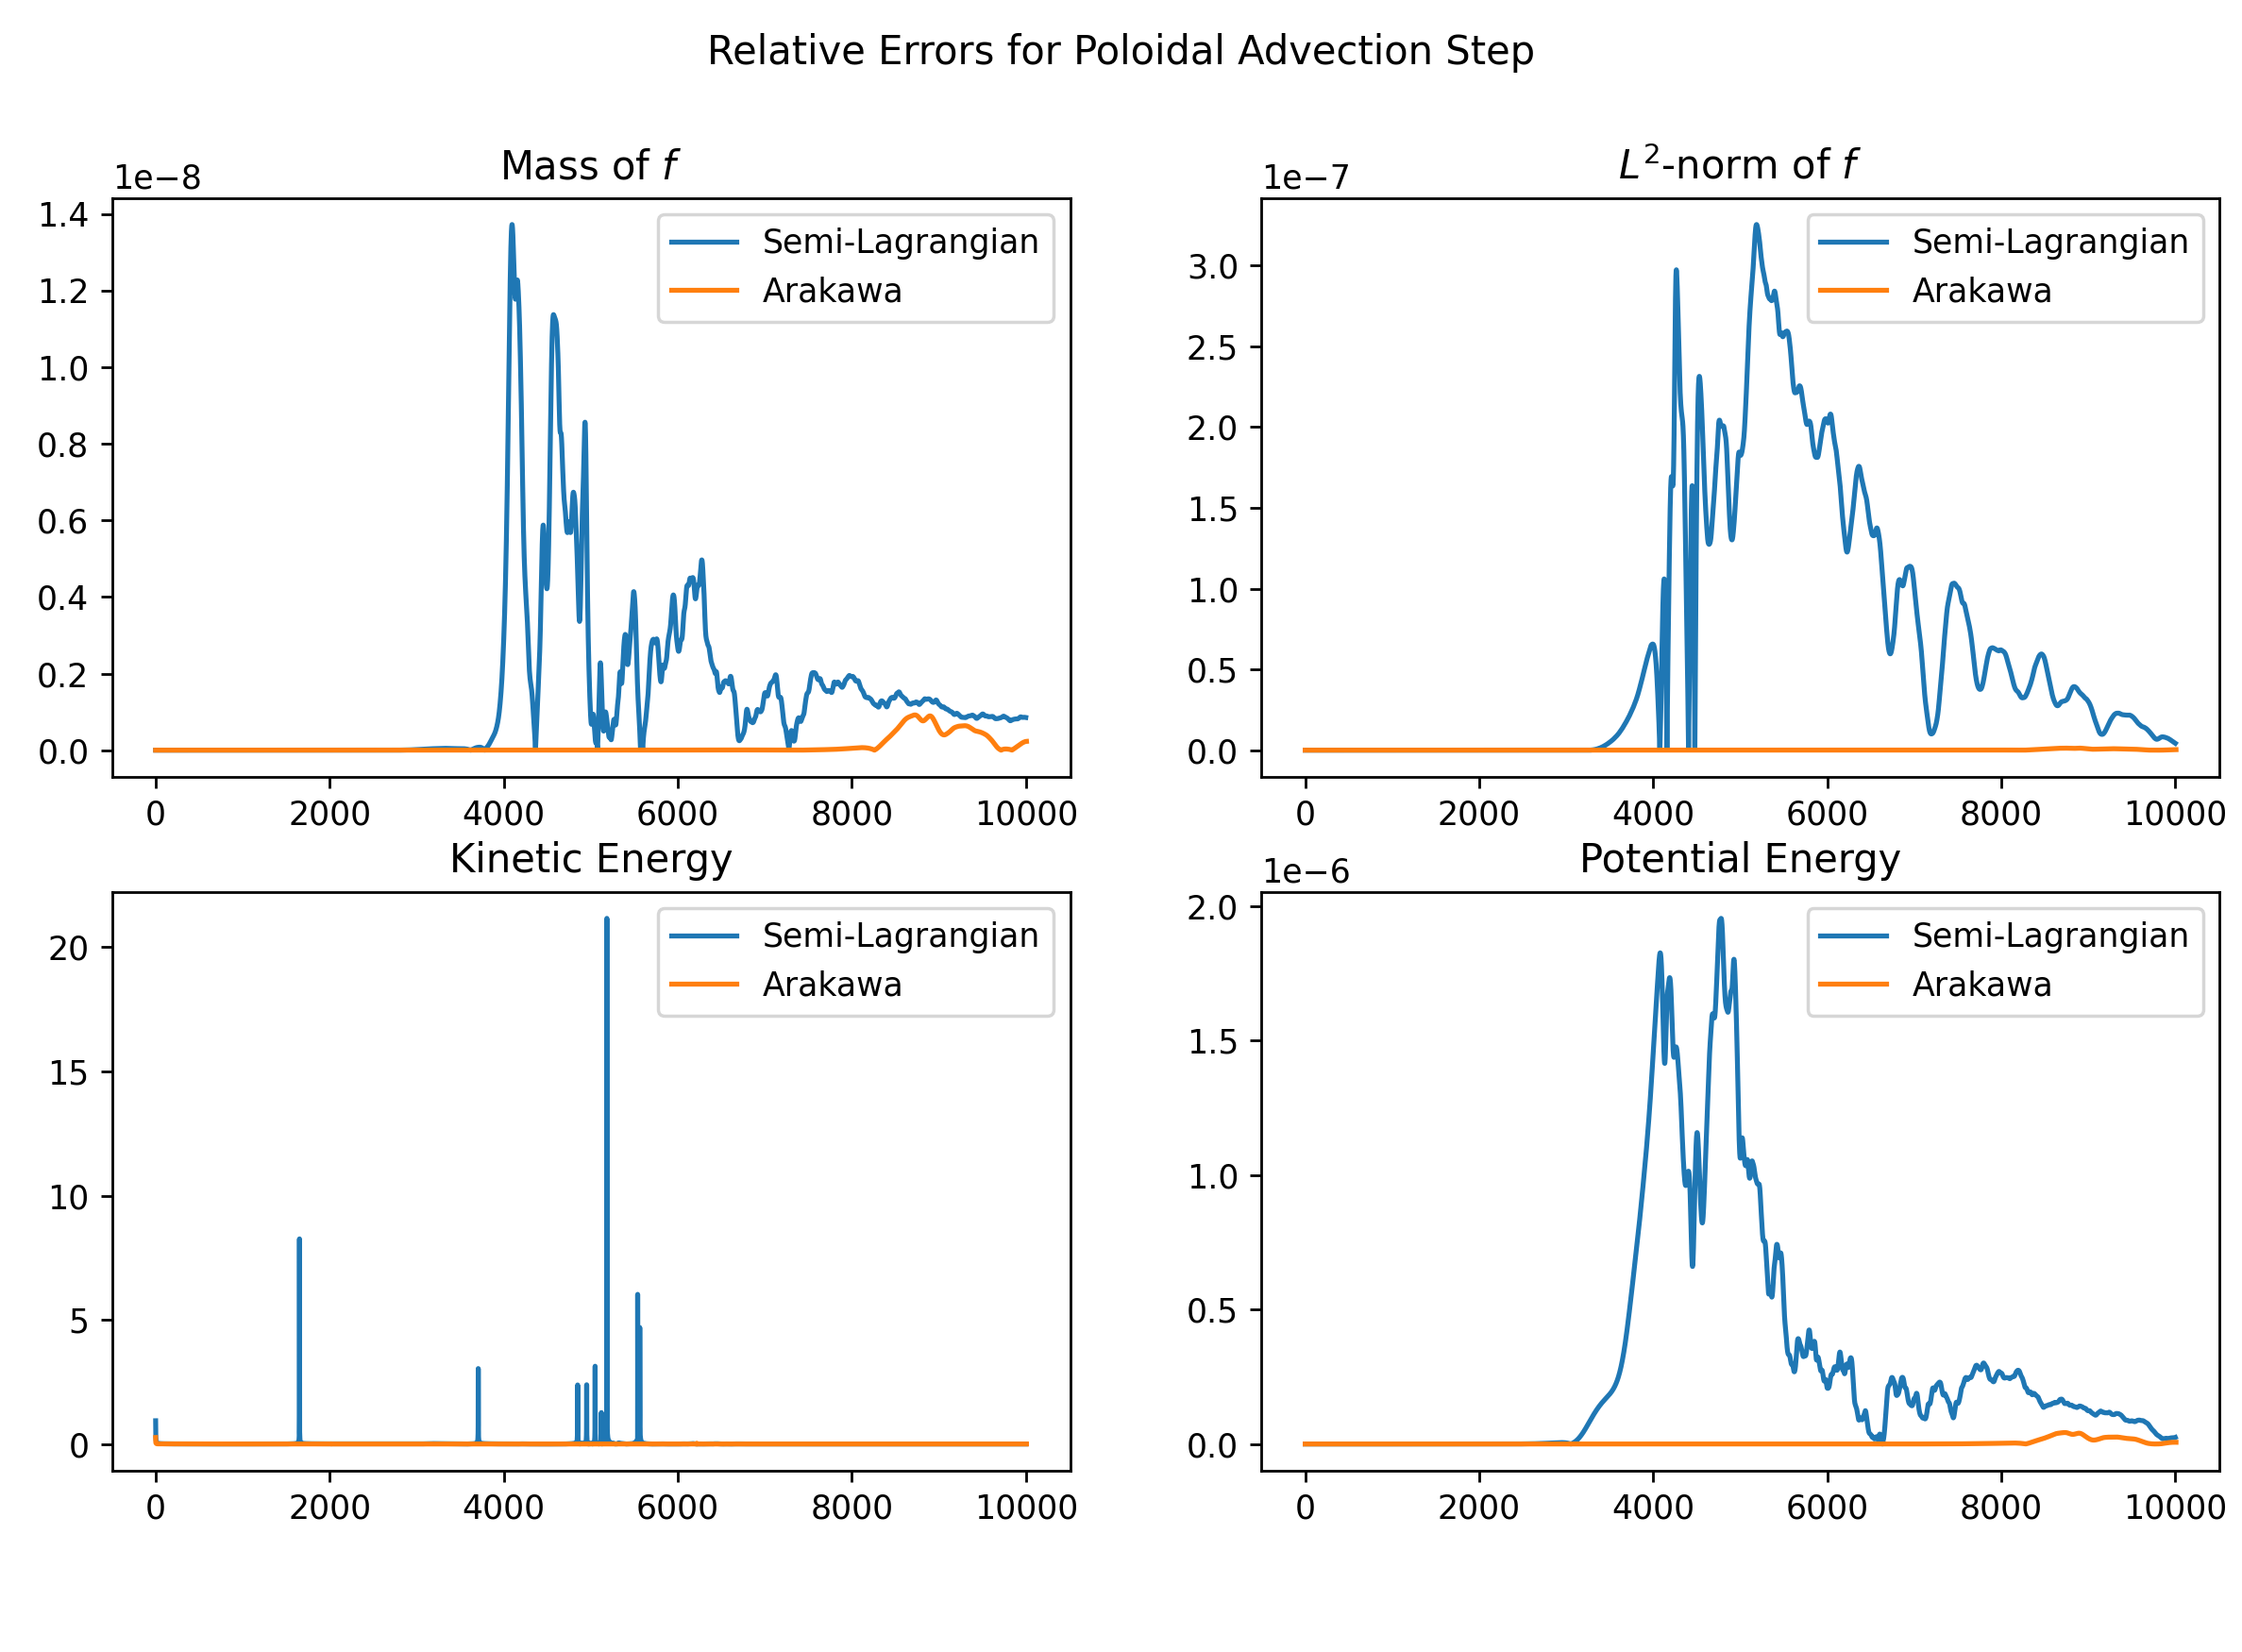
\includegraphics[width=0.9\linewidth]{plots/rel_err}
	\caption{The relative error for different quantities before and after the poloidal advection step.}
	\label{fig:relerr}
\end{figure}


\begin{figure}
	\centering
	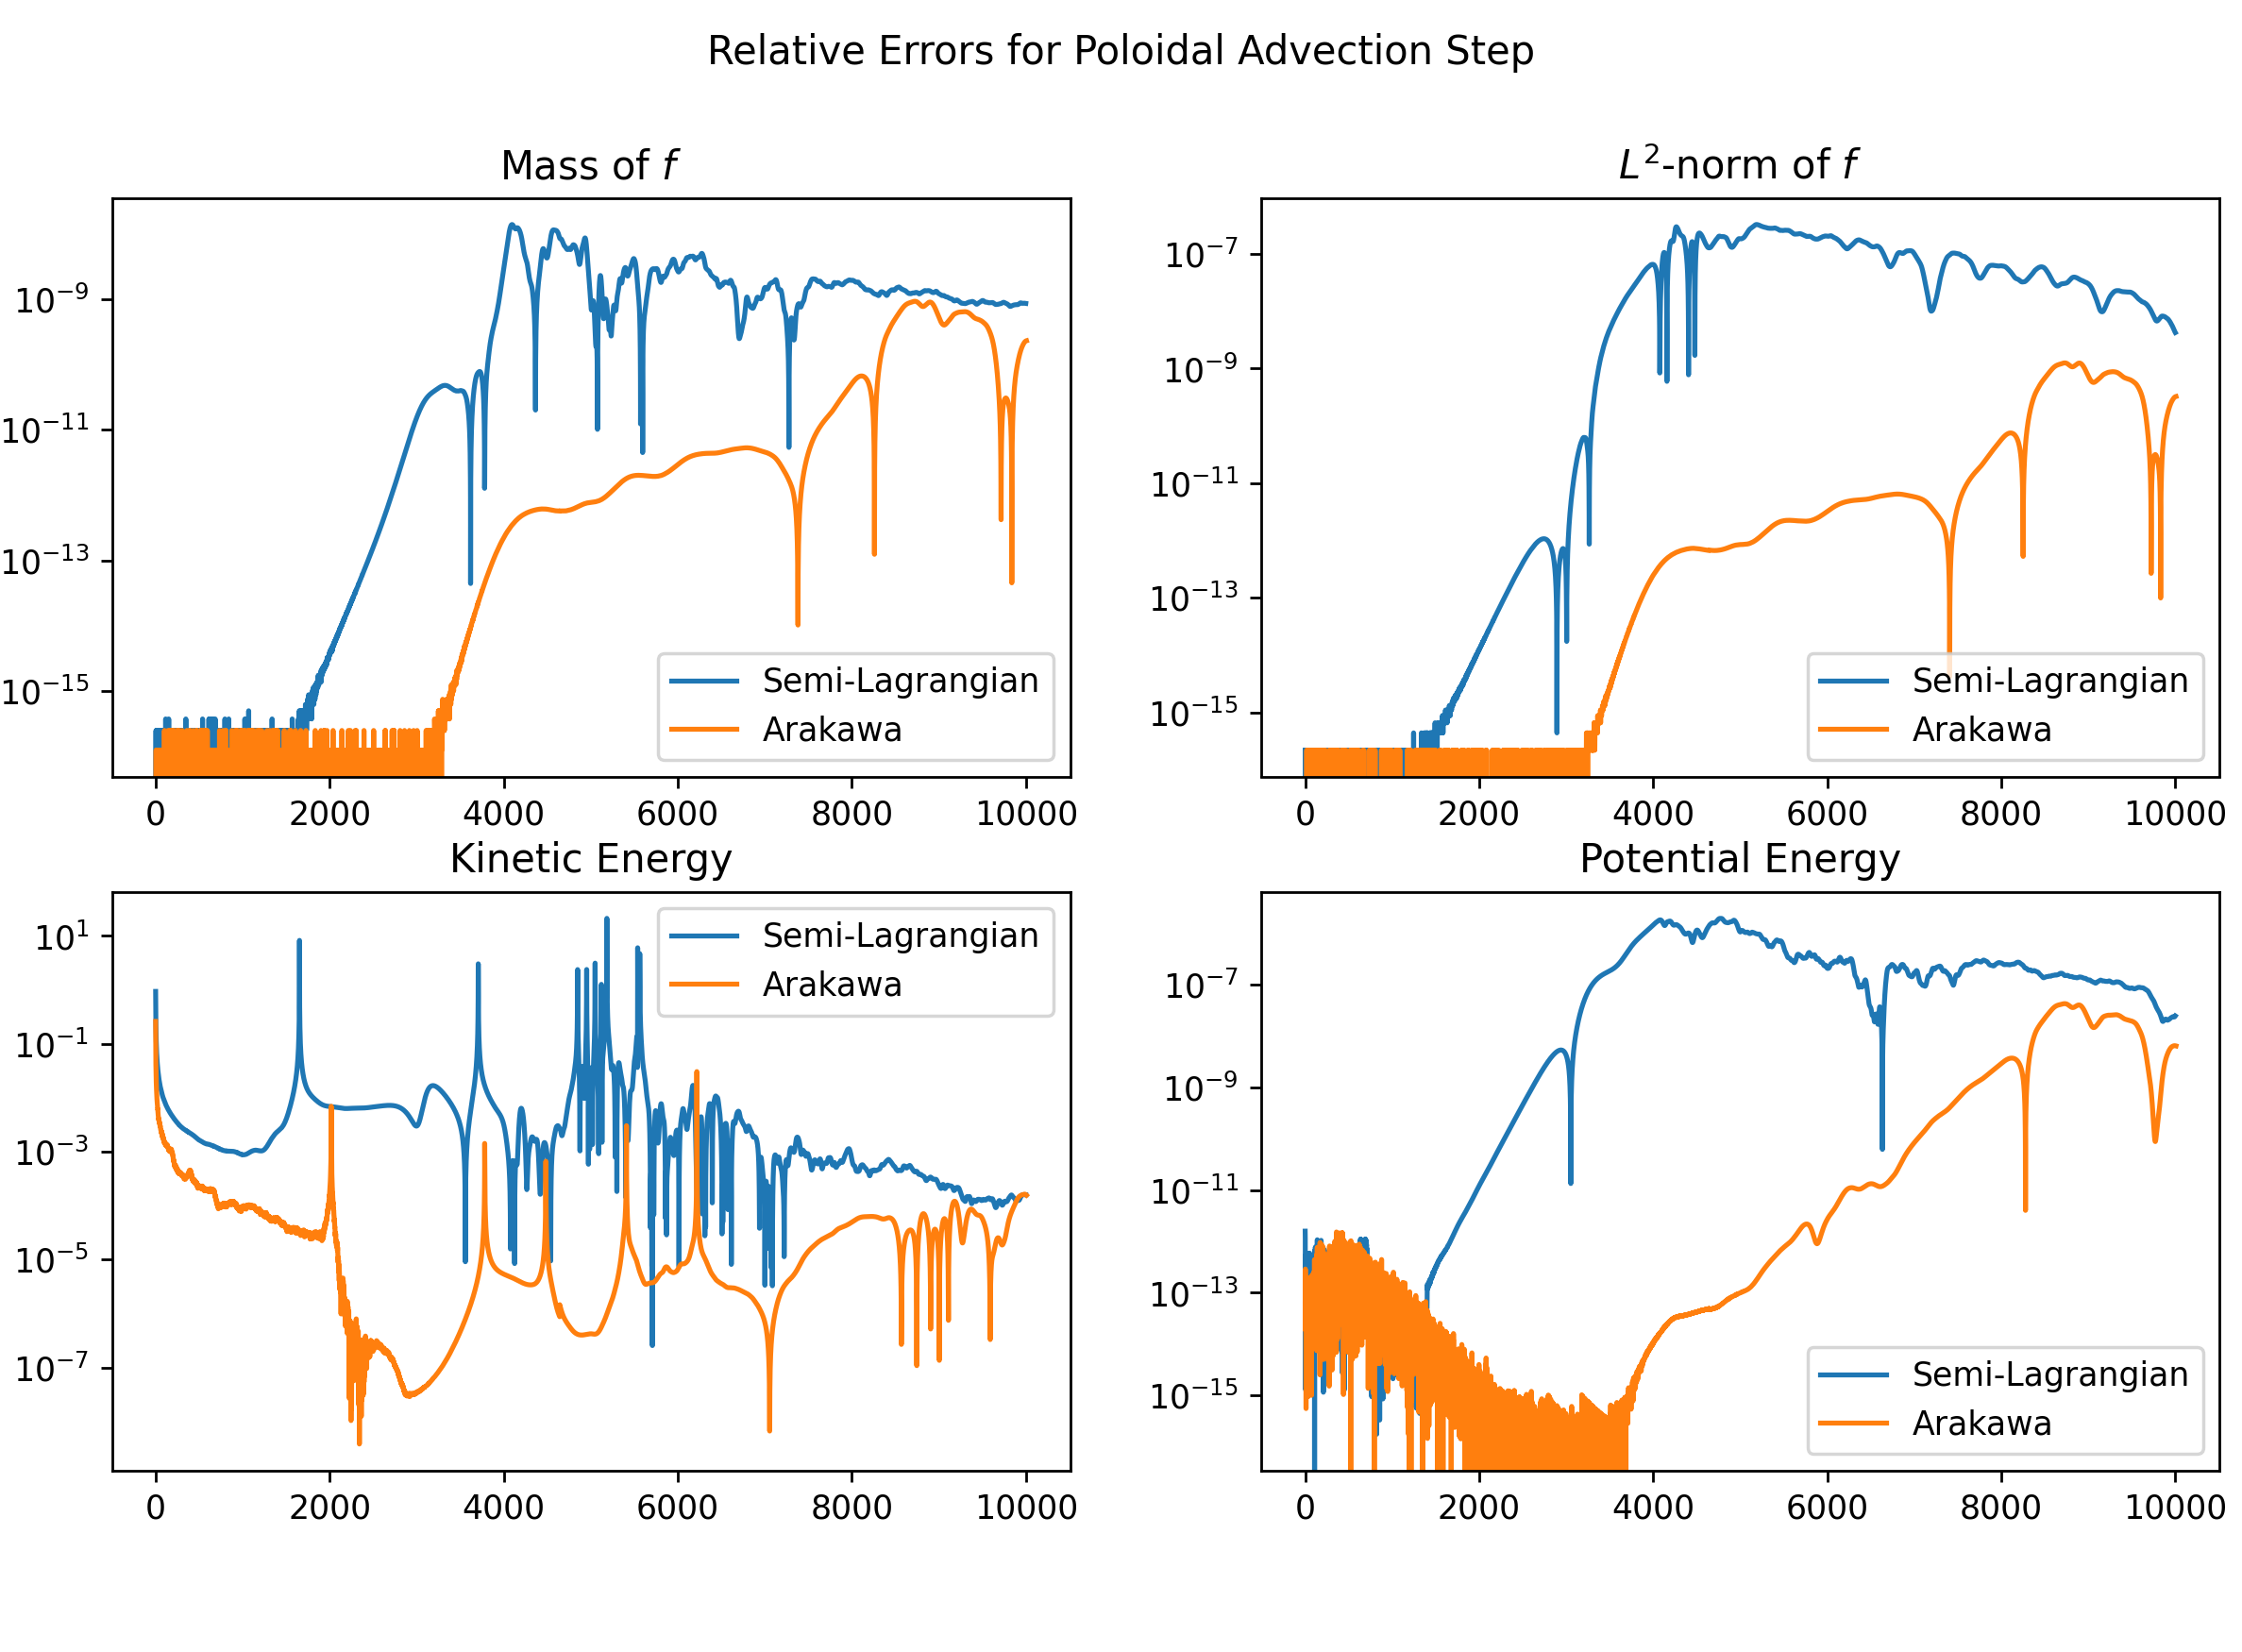
\includegraphics[width=0.9\linewidth]{plots/rel_err_log}
	\caption{The relative error for different quantities before and after the poloidal advection step on a semi-logarithmic scale.}
	\label{fig:relerrlog}
\end{figure}


\begin{figure}
	\centering
	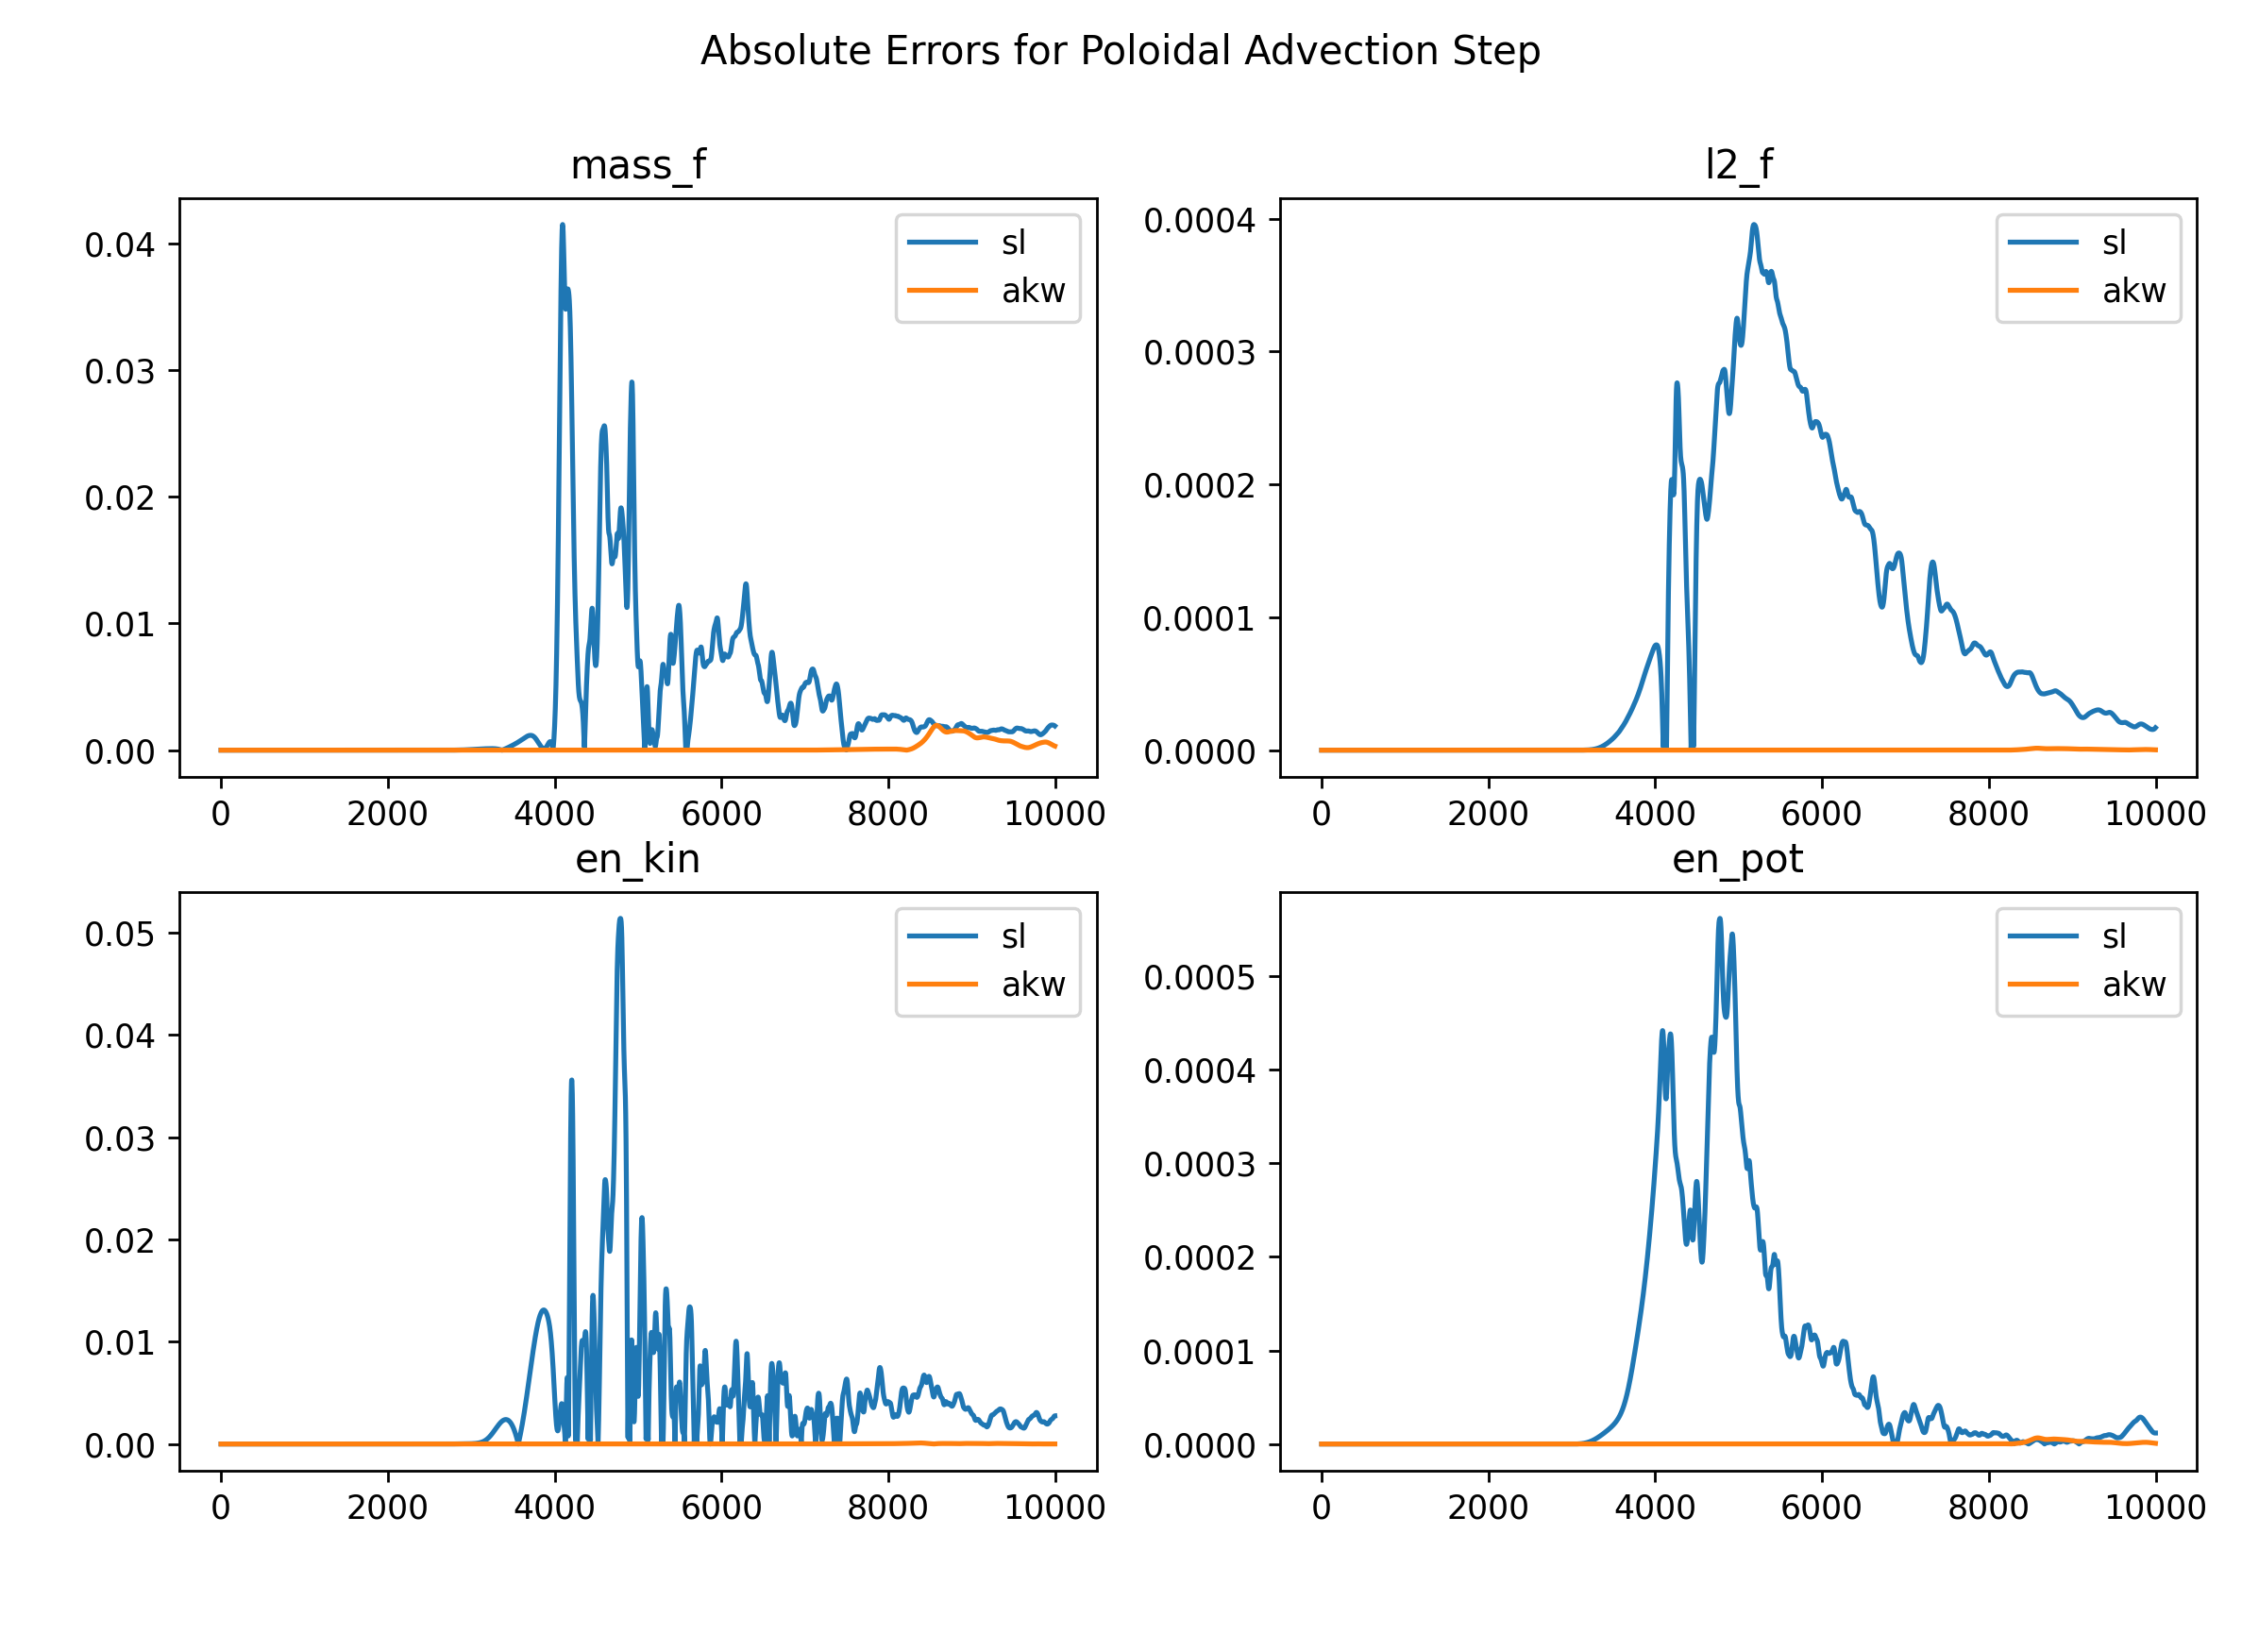
\includegraphics[width=0.9\linewidth]{plots/abs_err dt2}
	\caption{The absolute error for different quantities before and after the poloidal advection step with time step-size $\Delta t = 2$.}
	\label{fig:abserr_dt2}
\end{figure}


\begin{figure}
	\centering
	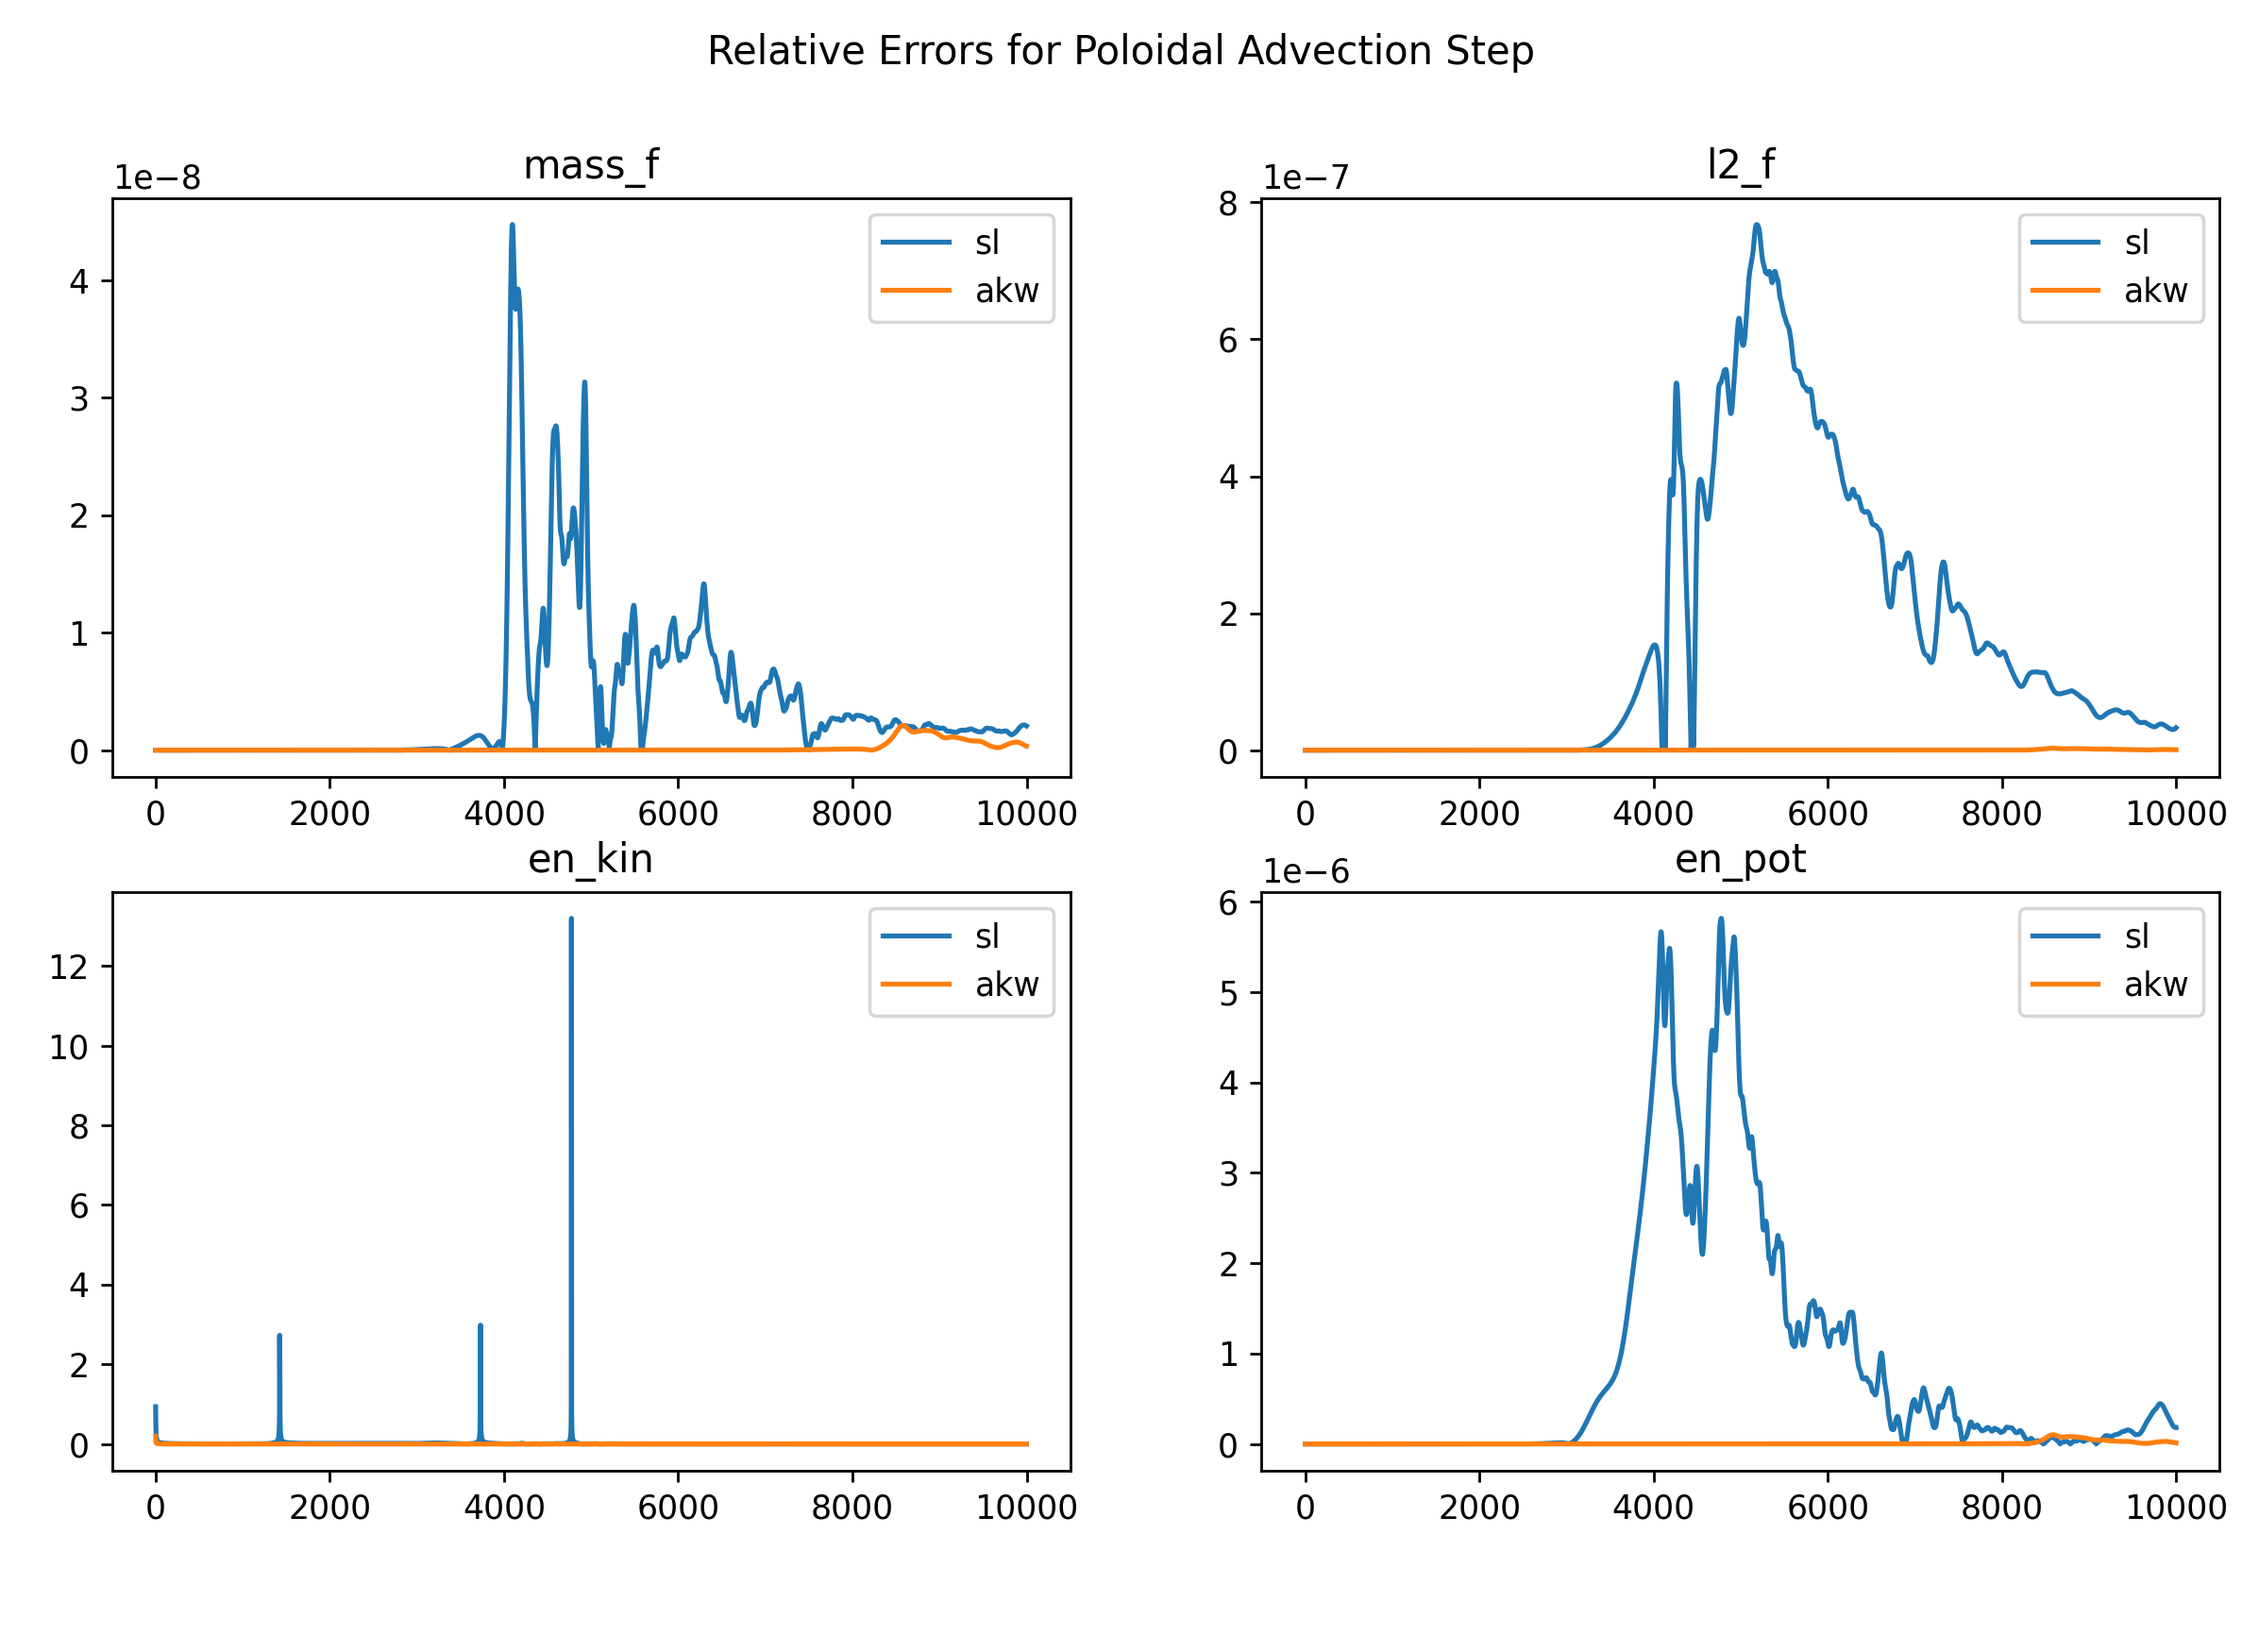
\includegraphics[width=0.9\linewidth]{plots/rel_err dt2}
	\caption{The relative error for different quantities before and after the poloidal advection step with time step-size $\Delta t = 2$.}
	\label{fig:relerr_dt2}
\end{figure}


\begin{figure}
	\centering
	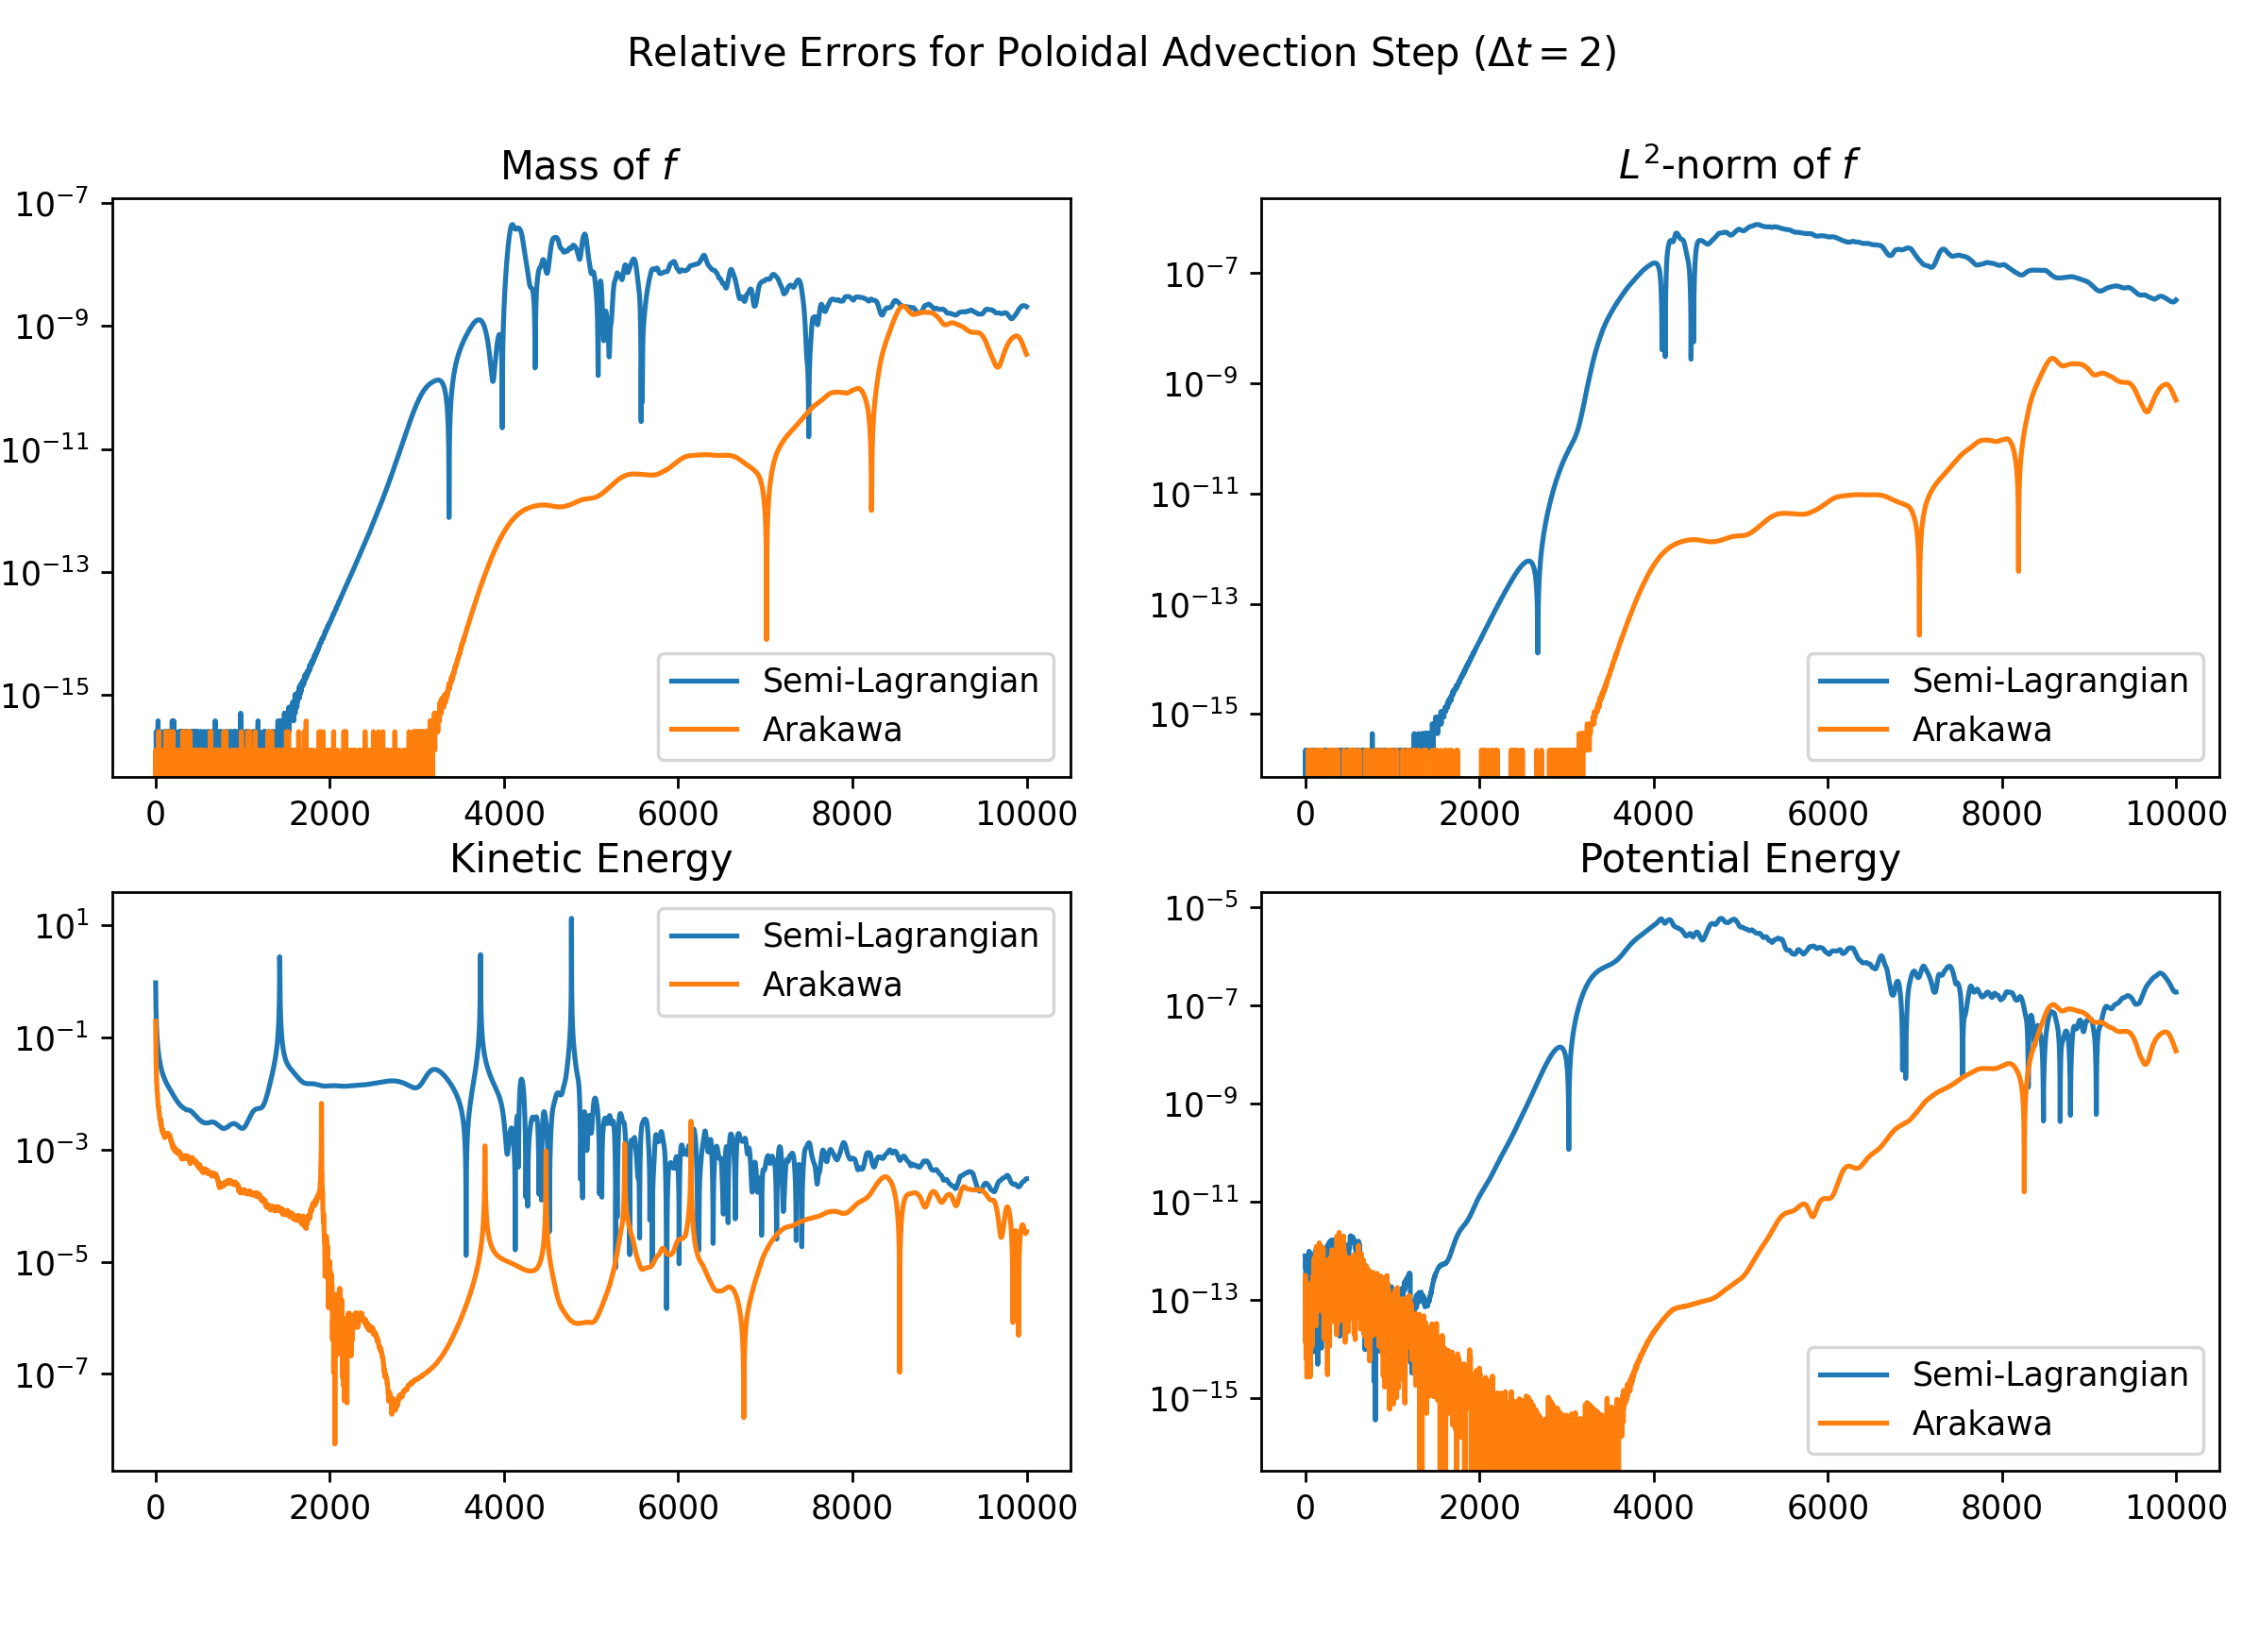
\includegraphics[width=0.9\linewidth]{plots/rel_err_log dt2}
	\caption{The relative error for different quantities before and after the poloidal advection step on a semi-logarithmic scale with time step-size $\Delta t = 2$.}
	\label{fig:relerrlog_dt2}
\end{figure}


\begin{figure}
	\centering
	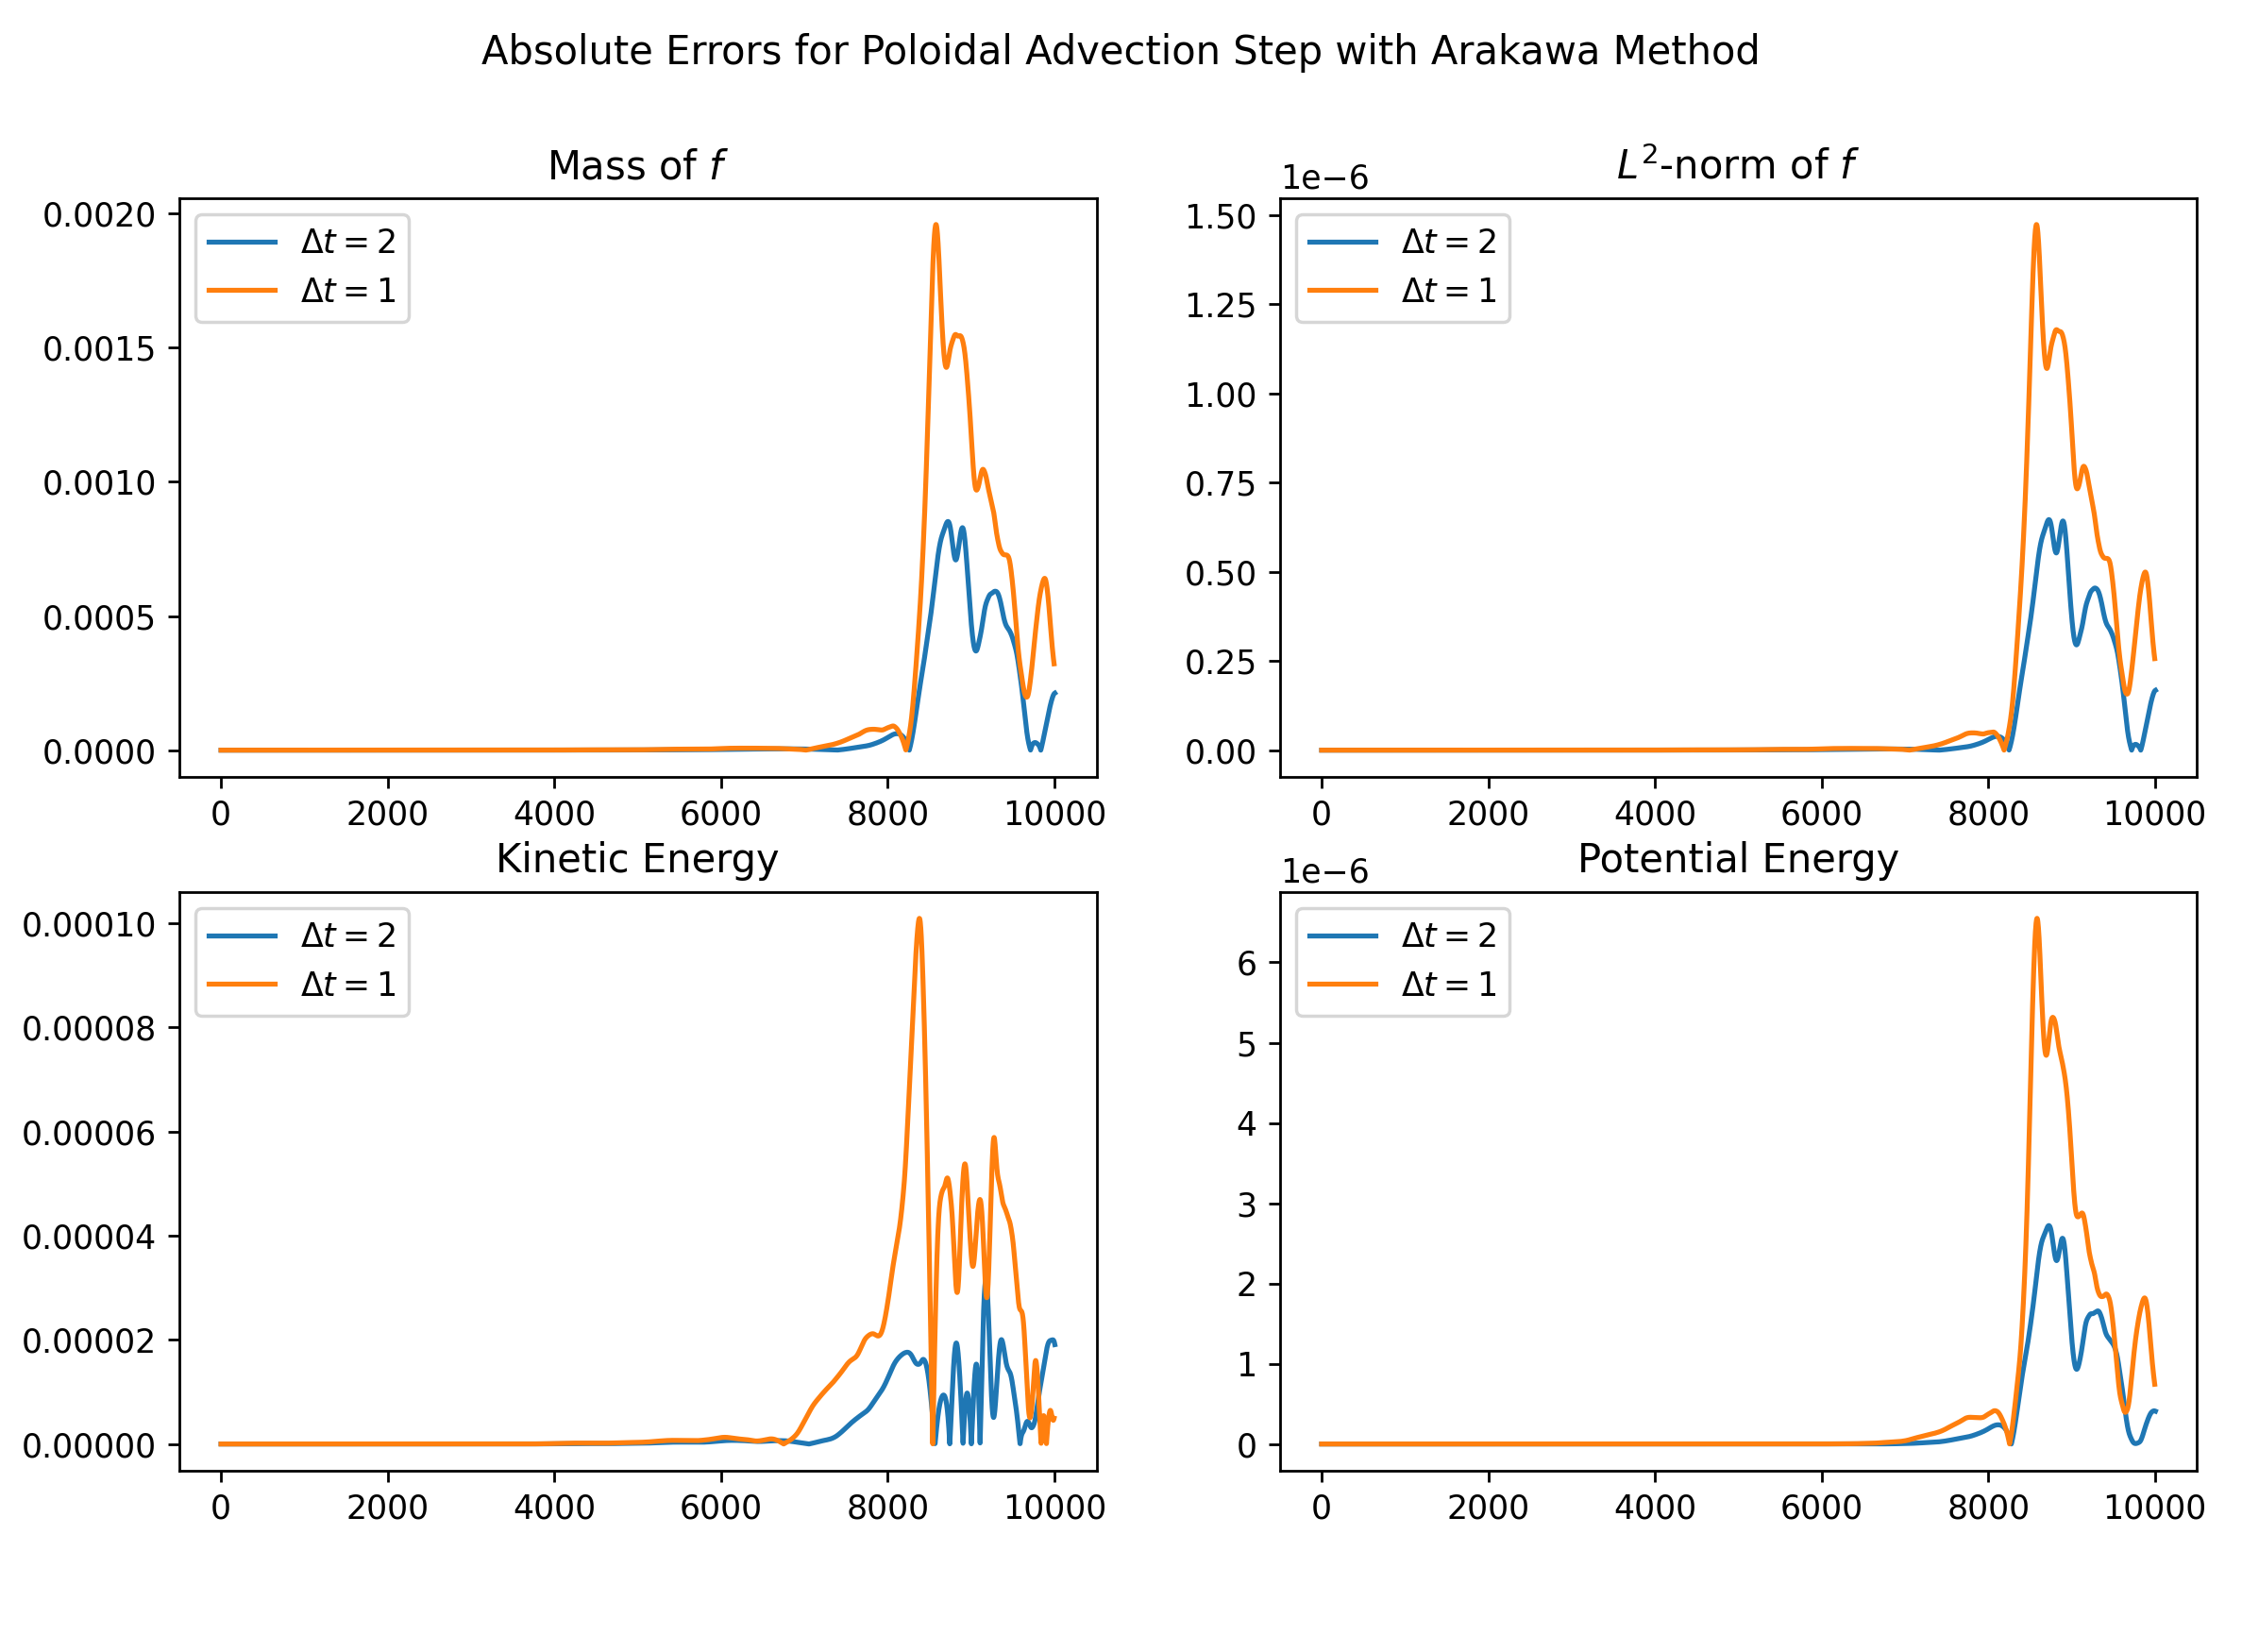
\includegraphics[width=0.9\linewidth]{plots/abs_err akw}
	\caption{The absolute error for different quantities before and after the poloidal advection step with the Arakawa method, comparing time step-size $\Delta t = 1$ and $\Delta t = 2$.}
	\label{fig:abserr_akw}
\end{figure}


\begin{figure}
	\centering
	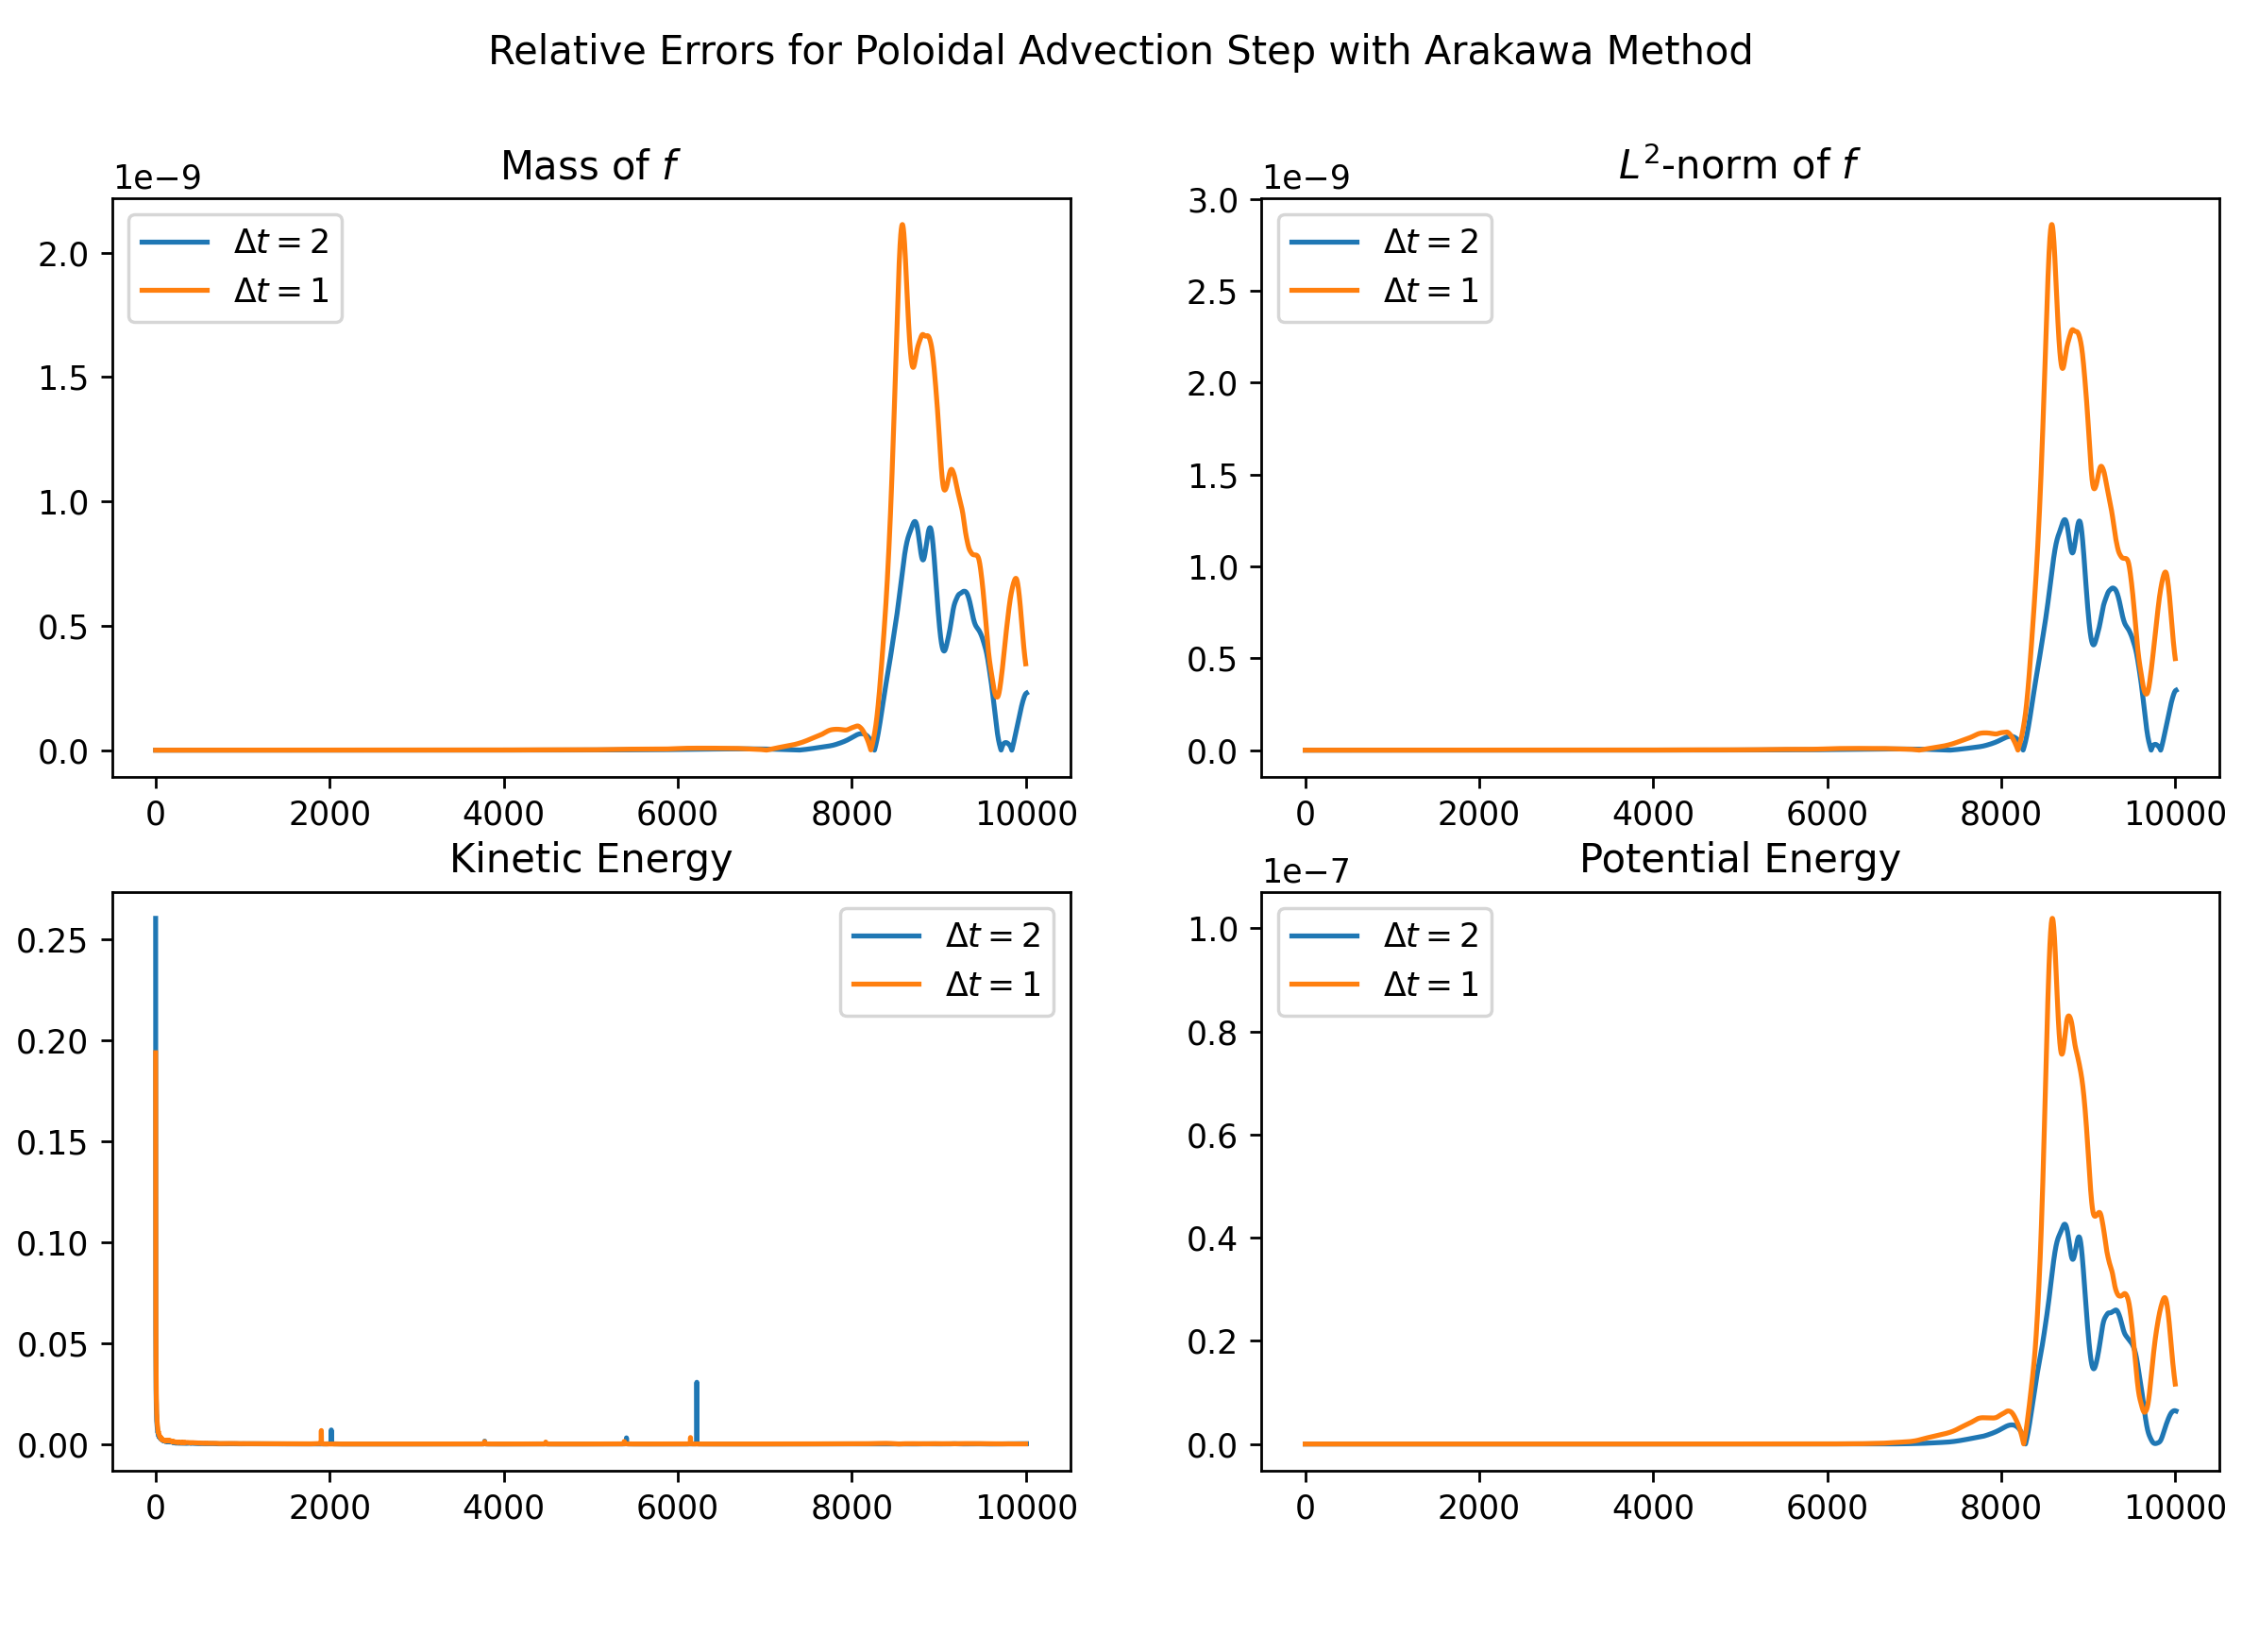
\includegraphics[width=0.9\linewidth]{plots/rel_err akw}
	\caption{The relative error for different quantities before and after the poloidal advection step with the Arakawa method, comparing time step-size $\Delta t = 1$ and $\Delta t = 2$..}
	\label{fig:relerr_akw}
\end{figure}


\begin{figure}
	\centering
	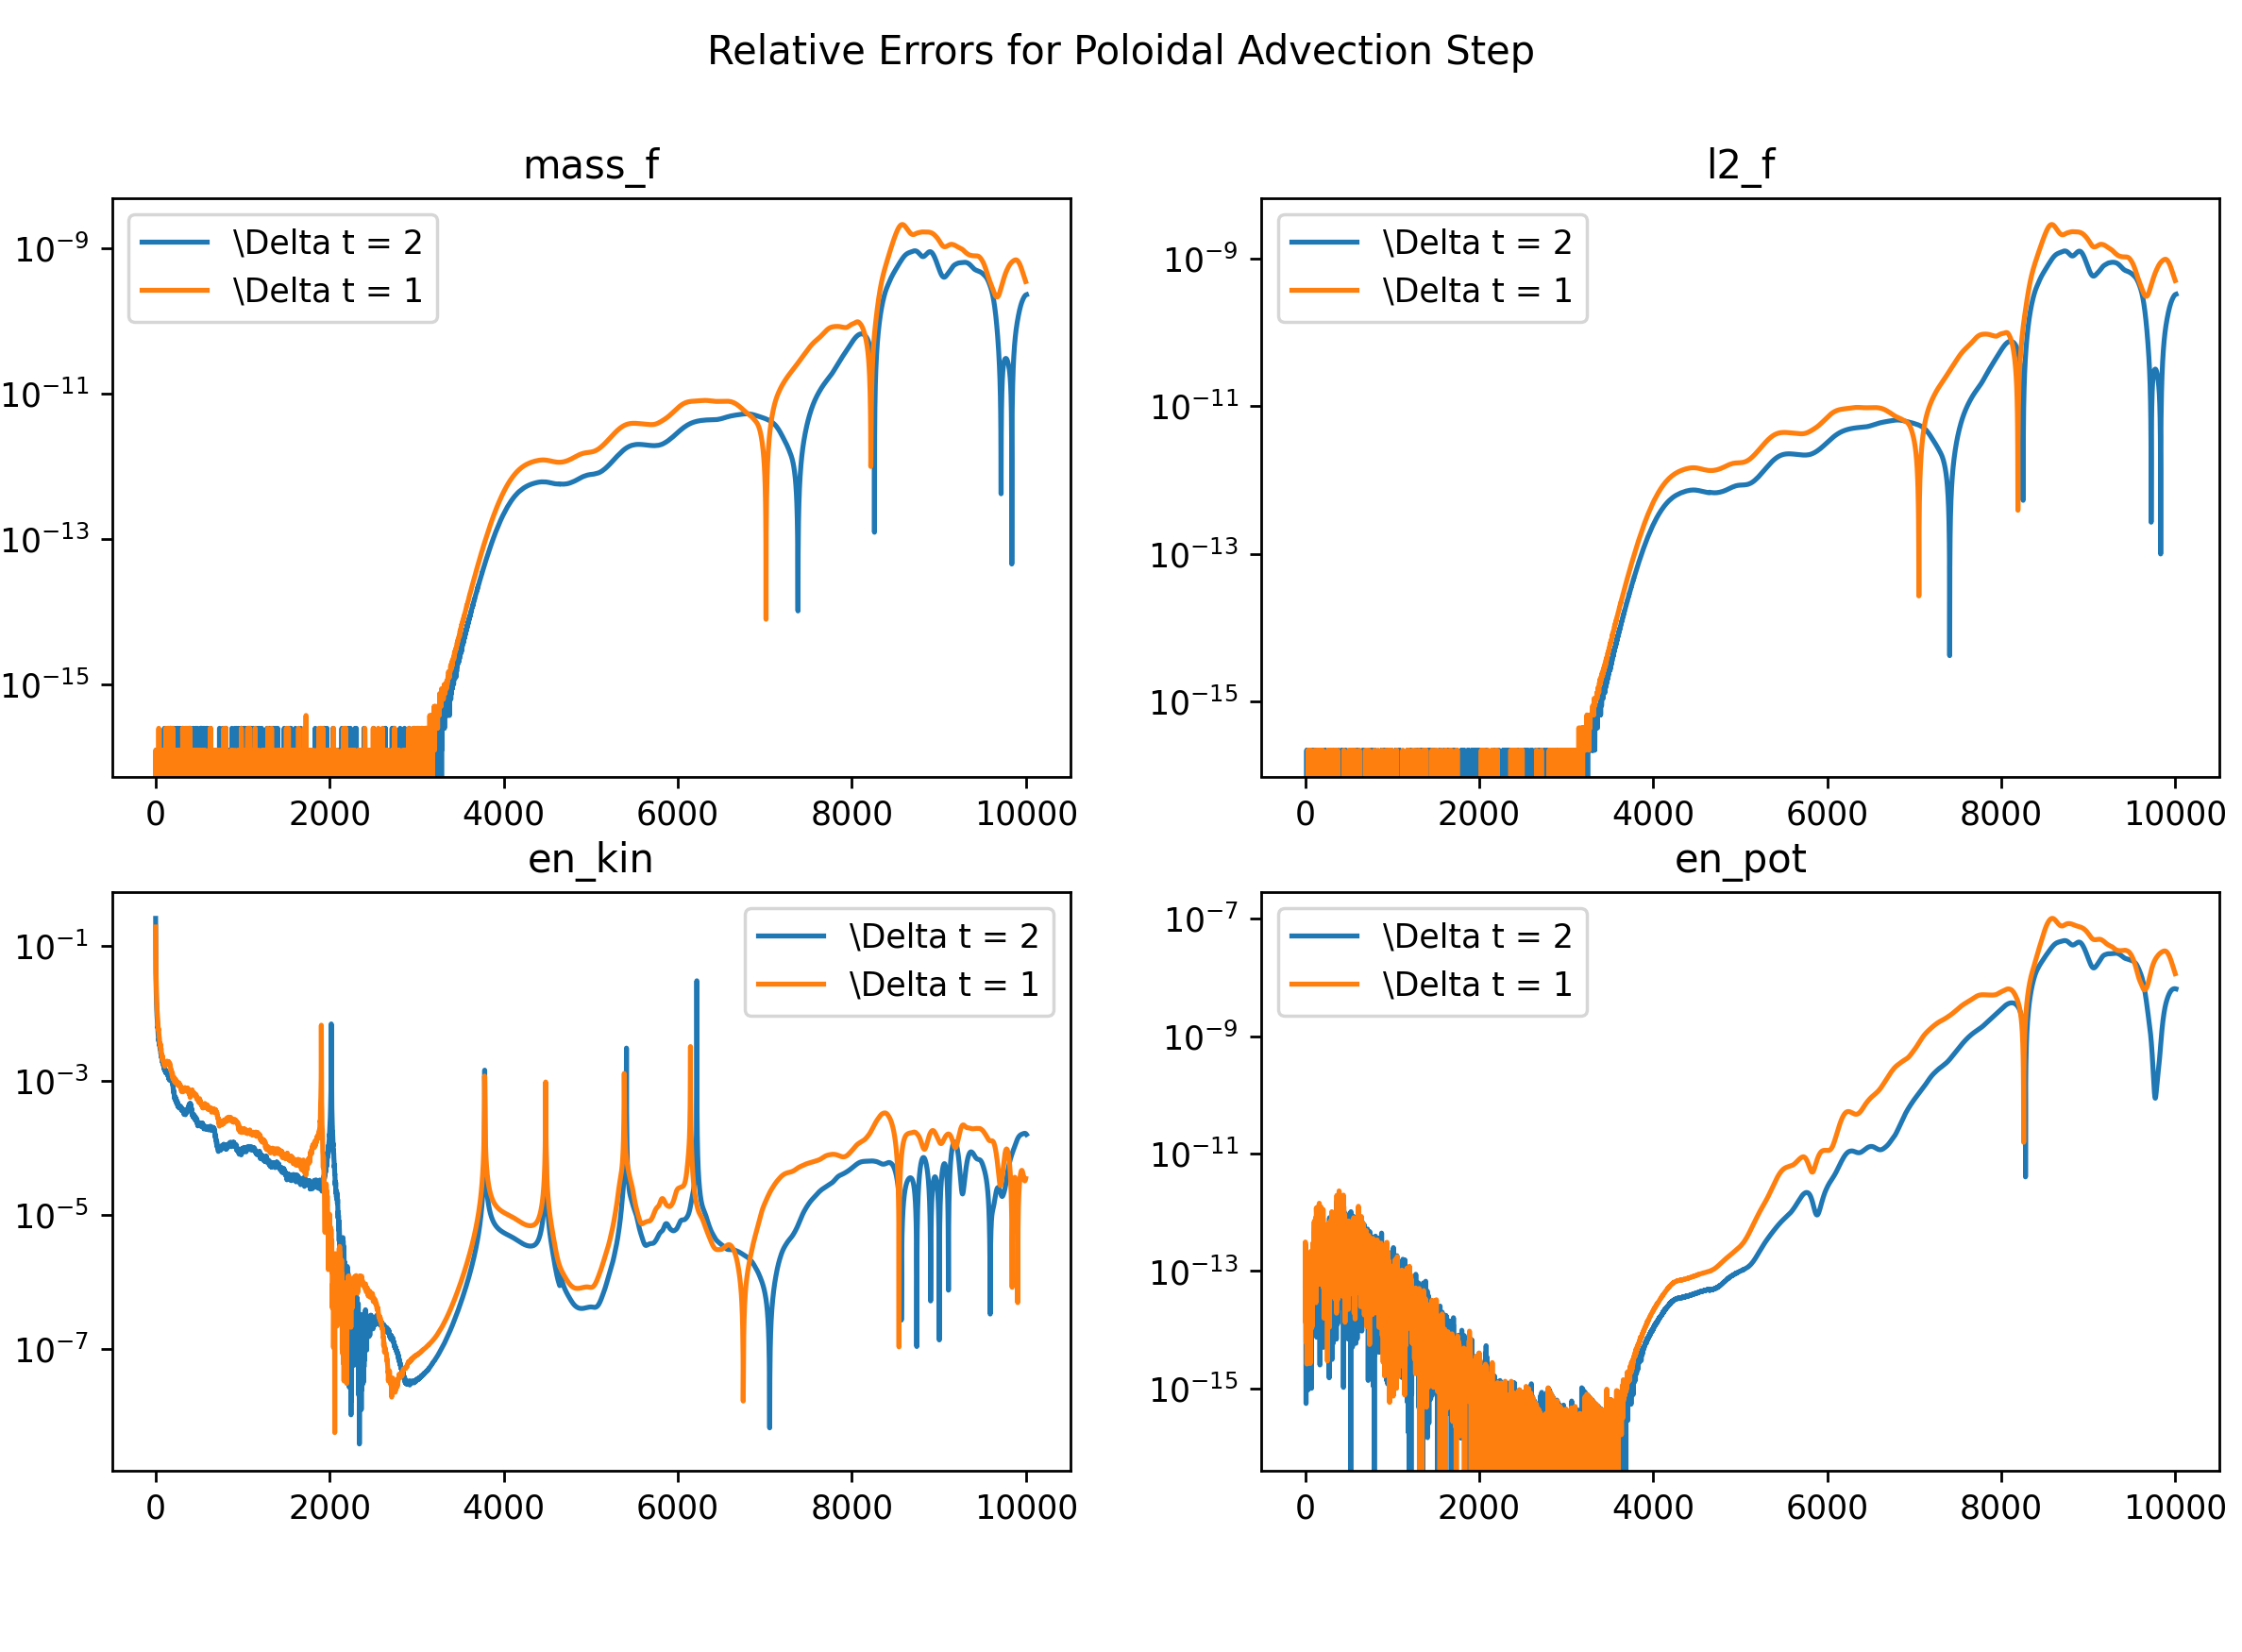
\includegraphics[width=0.9\linewidth]{plots/rel_err_log akw}
	\caption{The relative error for different quantities before and after the poloidal advection step on a semi-logarithmic scale with the Arakawa method, comparing time step-size $\Delta t = 1$ and $\Delta t = 2$..}
	\label{fig:relerrlog_akw}
\end{figure}





\appendix
% !TeX spellcheck = en_GB


\section{Order of Convergence for the Arakawa Scheme}
\label{sec:ara_order}

In order to calculate the convergence order of the different Finite Difference schemes, we use Mathematica and define the series expansion at every grid-point used in the stencil. Then introducing the discrete Jacobians, that will approximate our Poisson bracket, we combine them to the full Arakawa scheme and look at the appearing orders. The Mathematica input is written in bold font, while the output is following after. \\ 

\noindent\(	\pmb{F[\text{i$\_$}, \text{j$\_$}] = \text{Series}[f[x+i*h,y+j*h], \{h,0, 3\}, \{h,0, 3\}] \ \text{//}\text{Normal};}\\
	\pmb{\Phi[\text{i$\_$}, \text{j$\_$}] = \text{Series}[\varphi[x+i*h,y+j*h], \{h,0, 3\}, \{h,0, 3\}] \ \text{//}\text{Normal};} \)
\textbf{Second order - nine-point-stencil:}\\
%todo fix alignment
\begin{align*}
	\pmb{J^{++} = }
	\pmb{ \frac{1}{4 h^2}}
	&\pmb{( (F[1, 0] - F[-1, 0])*(\Phi[0,1]-\Phi[0,-1]) } \\
	&\pmb{- (F[0,1]-F[0,-1])*(\Phi[1,0]-\Phi[-1,0])) \ \text{//}\text{Simplify}};\\
%
	\pmb{J^{+x} = }
	\pmb{ \frac{1}{4 h^2}}
	&\pmb{( F[1,0]*(\Phi[1,1] - \Phi[1,-1])-F[-1, 0]*(\Phi[-1, 1]- \Phi[-1, -1]) - }\\
	&\pmb{F[0, 1]*(\Phi[1, 1] - \Phi[-1, 1]) + }
	\pmb{F[0, -1]*(\Phi[1, -1]-\Phi[-1,-1])) \ \text{//}\text{Simplify}}; \\
%
	\pmb{J^{x+} = }
	\pmb{ \frac{1}{4 h^2}}
	&\pmb{(F[1,1]*(\Phi[0,1]-\Phi[1,0])-F[-1,-1]*(\Phi[-1,0]-\Phi[0,-1]) }\\
	&-\pmb{F[-1,1]*(\Phi[0,1]-\Phi[-1,0])+F[1,-1]*(\Phi[1,0]-\Phi[0,-1])) \ \text{//}} \pmb{\text{Simplify}};\\
%
	\pmb{ J = \frac{1}{3}} & \pmb{(J^{++} + J^{+x} + J^{x+}) \ \text{//}\text{Simplify}};
\end{align*}
\begin{align*}
&\pmb{	\text{Collect}[J,h] } \ \text{//}\text{Simplify} \\
 &f^{(1,0)}(x,y) \varphi^{(0,1)}(x,y)-f^{(0,1)}(x,y) \varphi^{(1,0)}(x,y) \\
 &+\frac{1}{6} h^2 \left(f^{(1,0)}(x,y) \varphi^{(0,3)}(x,y)+f^{(1,0)}(x,y) \varphi^{(2,1)}(x,y)-f^{(0,3)}(x,y) \varphi^{(1,0)}(x,y) \right.\\
   &+f^{(1,1)}(x,y) \varphi^{(0,2)}(x,y)-f^{(0,2)}(x,y) \varphi^{(1,1)}(x,y)-f^{(0,1)}(x,y) \varphi^{(1,2)}(x,y)+f^{(2,0)}(x,y) \varphi^{(1,1)}(x,y)\\
   &-f^{(1,1)}(x,y) \varphi^{(2,0)}(x,y)-f^{(2,1)}(x,y)\varphi^{(1,0)}(x,y)\\
   &+\left.\left(f^{(1,2)}(x,y)+f^{(3,0)}(x,y)\right) \varphi^{(0,1)}(x,y)-f^{(0,1)}(x,y) \varphi^{(3,0)}(x,y)\right)\\
   &+ \frac{1}{36} h^4 \left(f^{(3,0)}(x,y) \varphi^{(2,1)}(x,y)+\left(f^{(1,2)}(x,y)+f^{(3,0)}(x,y)\right) \varphi^{(0,3)}(x,y) \right.\\
   &-\left.f^{(2,1)}(x,y) \varphi^{(3,0)}(x,y)-f^{(0,3)}(x,y) \left(\varphi^{(1,2)}(x,y)+\varphi^{(3,0)}(x,y)\right)\right)
\end{align*}

\newpage
\textbf{Fourth order - fourteen-point-stencil:}\\
\begin{align*}
\pmb{J^{xx} = \frac{1}{8h^2}} &\pmb{((F[1,1]-F[-1,-1])*(\Phi[-1,1]-\Phi[1,-1])} \\
	&\pmb{-(F[-1,1]-F[1,-1])*(\Phi[1,1]-\Phi	[-1,-1])) \ \text{//}\text{Simplify}}\\
	%
\pmb{J_2^{x+} =  \frac{1}{8h^2}}&\pmb{( F[1,1]*(\Phi[0,2] - \Phi[2, 0]) - F[-1,-1]*(\Phi[-2,0]-\Phi[0,-2])} \\
	&\pmb{-F[-1,1]*(\Phi[0,2]-\Phi[-2,0]) + F[1,-1]*(\Phi[2,0]-\Phi[0,-2])) \ \text{//}\text{Simplify}}\\
%
\pmb{J_2^{+x} =  \frac{1}{8h^2}}&\pmb{( F[2,0]*(\Phi[1,1] - \Phi[1, -1]) - F[-2,-0]*(\Phi[-1,1]-\Phi[-1,-1])}\\
&\pmb{- F[0,2]*(\Phi[1,1]-\Phi[-1,1]) + F[0,-2]*(\Phi[1,-1]-\Phi[-1,-1])) \ \text{//}}
\pmb{\text{Simplify}}\\
%
\pmb{J_2 = \frac{1}{3}}&\pmb{(J^{xx}+J_2^{x+}+J_2^{+x}) \ \text{//}\text{Simplify}}\\
%
\pmb{J' = 2J }&\pmb{-J_2 \text{//}\text{Simplify}}
\end{align*}
\begin{align*}
&\pmb{	\text{Collect}[J',h] } \ \text{//}\text{Simplify} \\
&f^{(1,0)}(x,y) \varphi^{(0,1)}(x,y)-f^{(0,1)}(x,y) \varphi^{(1,0)}(x,y) \\
&+ \frac{1}{36} h^4 \left(\left(3 f^{(1,2)}(x,y)+f^{(3,0)}(x,y)\right)\left(-\varphi^{(0,3)}(x,y)\right) +f^{(0,3)}(x,y) \left(3 \varphi^{(1,2)}(x,y)+\varphi^{(3,0)}(x,y)\right) \right.\\
&+3 \left(f^{(2,1)}(x,y) \varphi^{(1,2)}(x,y)+f^{(2,1)}(x,y) \varphi^{(3,0)}(x,y) - \left. f^{(1,2)}(x,y) \varphi^{(2,1)}(x,y)-f^{(3,0)}(x,y) \varphi^{(2,1)}(x,y)\right)\right)
\end{align*}



\begin{acknowledgement}
	Acknowledgement to the people, thanks to the institutions (in the title)...
\end{acknowledgement}

\bibliographystyle{ieeetr}
\bibliography{literature}
\end{document}
